%%%%%%%%%%%%%%%%%%%%%%%%%%%%%%%%%%%%%%%%%
% Masters/Doctoral Thesis 
% LaTeX Template
% Version 2.4 (22/11/16)
%
% This template has been downloaded from:
% http://www.LaTeXTemplates.com
%
% Version 2.x major modifications by:
% Vel (vel@latextemplates.com)
%
% This template is based on a template by:
% Steve Gunn (http://users.ecs.soton.ac.uk/srg/softwaretools/document/templates/)
% Sunil Patel (http://www.sunilpatel.co.uk/thesis-template/)
%
% Template license:
% CC BY-NC-SA 3.0 (http://creativecommons.org/licenses/by-nc-sa/3.0/)
%
%%%%%%%%%%%%%%%%%%%%%%%%%%%%%%%%%%%%%%%%%

%----------------------------------------------------------------------------------------
%	PACKAGES AND OTHER DOCUMENT CONFIGURATIONS
%----------------------------------------------------------------------------------------

\documentclass[
11pt, % The default document font size, options: 10pt, 11pt, 12pt
oneside, % Two side (alternating margins) for binding by default, uncomment to switch to one side
%catalan,
english,
%spanish,
singlespacing, % Single line spacing, alternatives: onehalfspacing or doublespacing
%draft, % Uncomment to enable draft mode (no pictures, no links, overfull hboxes indicated)
%nolistspacing, % If the document is onehalfspacing or doublespacing, uncomment this to set spacing in lists to single
%liststotoc, % Uncomment to add the list of figures/tables/etc to the table of contents
%toctotoc, % Uncomment to add the main table of contents to the table of contents
%parskip, % Uncomment to add space between paragraphs
%nohyperref, % Uncomment to not load the hyperref package
headsepline, % Uncomment to get a line under the header
%chapterinoneline, % Uncomment to place the chapter title next to the number on one line
%consistentlayout, % Uncomment to change the layout of the declaration, abstract and acknowledgements pages to match the default layout
]{MastersDoctoralThesis} % The class file specifying the document structure

\usepackage[utf8]{inputenc} % Required for inputting international characters
\usepackage[T1]{fontenc} % Output font encoding for international characters
\usepackage{eurosym}
\usepackage{footnote}
\usepackage{palatino} % Use the Palatino font by default
\usepackage{babel}
\usepackage[backend=bibtex,style=numeric,natbib=true,sorting=none]{biblatex}
\usepackage{multirow}
\usepackage{float}
\usepackage{tabularx}
\usepackage{listings}
\usepackage{xcolor}
\usepackage{appendix}
\usepackage{datetime}
\usepackage{array}
\usepackage{mathtools}
\usepackage{colortbl}
%\usepackage{wrapfig}
%\usepackage{fontspec}
%\setmainfont{Helvetica Neue Light}

\addbibresource{main.bib} % The filename of the bibliography

\usepackage[autostyle=true]{csquotes} % Required to generate language-dependent quotes in the bibliography

\newdate{date}{15}{06}{2018}
\date{\displaydate{date}}

%----------------------------------------------------------------------------------------
%	MARGIN SETTINGS
%----------------------------------------------------------------------------------------

\geometry{
	paper=a4paper, % Change to letterpaper for US letter
	inner=2.5cm, % Inner margin
	outer=3cm, % Outer margin
	bindingoffset=.5cm, % Binding offset
	top=1.5cm, % Top margin
	bottom=1.5cm, % Bottom margin
	%showframe, % Uncomment to show how the type block is set on the page
}

%----------------------------------------------------------------------------------------
%	THESIS INFORMATION
%----------------------------------------------------------------------------------------

\thesistitle{Skyscanner offer and demand comparison} % Your thesis title, this is used in the title and abstract, print it elsewhere with \ttitle
\supervisor{Javier Arias} % Your supervisor's name, this is used in the title page, print it elsewhere with \supname
\examiner{} % Your examiner's name, this is not currently used anywhere in the template, print it elsewhere with \examname
\degree{Computer Engineering Degree} % Your degree name, this is used in the title page and abstract, print it elsewhere with \degreename
\author{Fèlix Arribas} % Your name, this is used in the title page and abstract, print it elsewhere with \authorname
\addresses{} % Your address, this is not currently used anywhere in the template, print it elsewhere with \addressname

\def \universitysupervisor{Maria José Casany}
\def \thesis{Skyscanner offer and demand comparison}

\keywords{} % Keywords for your thesis, this is not currently used anywhere in the template, print it elsewhere with \keywordnames
\university{Universitat Politècnica de Catalunya (UPC)} % Your university's name and URL, this is used in the title page and abstract, print it elsewhere with \univname
\department{\href{https://www.essi.upc.edu/}{Software Engineering and Information Systems department}} % Your department's name and URL, this is used in the title page and abstract, print it elsewhere with \deptname
\group{\href{https://www.essi.upc.edu/}{ESSI}} % Your research group's name and URL, this is used in the title page, print it elsewhere with \groupname
\faculty{\href{http://www.fib.upc.edu}{Facultat d'Informàtica de Barcelona (FIB)}} % Your faculty's name and URL, this is used in the title page and abstract, print it elsewhere with \facname

\def \company{Skyscanner}
\def \tribe{Marketplace Engine tribe}
\def \squad{DeLorean squad}

\AtBeginDocument{
\hypersetup{pdftitle=\ttitle} % Set the PDF's title to your title
\hypersetup{pdfauthor=\authorname} % Set the PDF's author to your name
\hypersetup{pdfkeywords=\keywordnames} % Set the PDF's keywords to your keywords
\hypersetup{linkcolor=black}
}

\newcolumntype{L}{>{\centering}m{0.75cm}}
\newcolumntype{M}{m{9cm}}
\newcolumntype{T}{m{12cm}}

\newcommand\tab[1][0.75cm]{\hspace*{#1}}
\newcommand*\NewPage{\newpage\null\thispagestyle{empty}\newpage}


\colorlet{punct}{red!60!black}
\definecolor{background}{HTML}{EEEEEE}
\definecolor{delim}{RGB}{20,105,176}
\colorlet{numb}{magenta!60!black}

\lstdefinelanguage{json}{
    basicstyle=\normalfont\ttfamily,
    numbers=left,
    numberstyle=\scriptsize,
    stepnumber=1,
    numbersep=8pt,
    showstringspaces=false,
    breaklines=true,
    frame=lines,
    backgroundcolor=\color{background}
}

\lstdefinelanguage{java}{
    basicstyle=\normalfont\ttfamily,
    numbers=left,
    numberstyle=\scriptsize,
    stepnumber=1,
    numbersep=8pt,
    showstringspaces=false,
    breaklines=true,
    frame=lines,
    backgroundcolor=\color{background}
}

\setlength{\parindent}{0pt}

\begin{document}
\selectlanguage{english}

\frontmatter % Use roman page numbering style (i, ii, iii, iv...) for the pre-content pages

\pagestyle{plain} % Default to the plain heading style until the thesis style is called for the body content

%----------------------------------------------------------------------------------------
%	TITLE
%----------------------------------------------------------------------------------------

\begin{titlepage}
\begin{center}


\includegraphics[scale=0.3]{resources/logo-skyscanner.png}


\includegraphics[scale=0.2]{resources/logo-upc.png} % University/department logo - uncomment to place it

\vspace*{.04\textheight}
{\scshape\LARGE \href{https://www.skyscanner.net/}{\company}\\ in collaboration with\\ \href{http://www.upc.edu}\univname\par}\vspace{1.5cm} % University name
\textsc{\Large Final Degree Project}\\[0.5cm] % Thesis type

\HRule \\[0.4cm] % Horizontal line
{\Huge \bfseries \ttitle\par}\vspace{0.4cm} % Thesis 
{\large Skyscanner available flights and user searches comparison\par}\vspace{0.1cm} % Thesis title
\HRule \\[1.5cm] % Horizontal line
 
\begin{minipage}[t]{0.4\textwidth}
\begin{flushleft} \large
\emph{Author:}\\
\authorname % Author name - remove the \href bracket to remove the link
\end{flushleft}
\end{minipage}
\begin{minipage}[t]{0.4\textwidth}
\begin{flushright} \large
\emph{Director:} \\
\supname % Supervisor name - remove the \href bracket to remove the link  
\\
\emph{University supervisor:} \\
\universitysupervisor
\end{flushright}
\end{minipage}\\[3cm]
 
\vfill

\large \textit{A Project for the}
\large \degreename 
\textit{ in the}\\[0.2cm]
\deptname\\[0.2cm]
\facname\\[0.2cm]
\textit{working with}\\[0.2cm]
\squad
\textit{ from}
\tribe\\
\vfill

{\large \displaydate{date}}\\[4cm] % Date
 
\vfill
\end{center}
\end{titlepage}
\NewPage

%----------------------------------------------------------------------------------------
%	ABSTRACT
%----------------------------------------------------------------------------------------

\begin{abstract}
\addchaptertocentry{\abstractname}
In the last century, the world has became smaller. Communications are easier and faster than fifty years ago. Back then, you could talk through a fix phone, but you were not able to send any kind of media, like photos, videos, etc. Only the latest technology of that moment was able to do that. Since the smart phone revolution in 2007 almost everyone can text messages, send images, share live videos and much more in less than a second.
\\\\
But the internet, phones and communications are not the only thing that made the world smaller. Ways of traveling helped that earth flattering too. In 1918 visiting another place was very difficult. If you wanted to cross the sea, you had to do it by boat, and those trips could last days or weeks. The fastest way to travel very far in a continent was by train, but not all places were connected with rails. Nowadays, all along with the internet revolution, anyone can travel to the other side of the world in less than a day by plane. Even for traveling inside the same country people use planes.
\\\\
But, is the air industry as efficient enough? Are all airlines' users satisfied with their purchases and possibilities? \company\ provides a user friendly tool to search cheap flights from any airport to another. Sadly, sometimes is difficult for users to find what they really want.
\\\\
This project wants to help to solve this problem, providing a visual comparison to explore differences and similarities between what the users search and what the airlines provide. Making easier to compare between specific dates to guess user behavior.
\end{abstract}

%----------------------------------------------------------------------------------------
%	TABLE OF CONTENTS
%----------------------------------------------------------------------------------------
\NewPage
\tableofcontents

%----------------------------------------------------------------------------------------
%   THESIS CONTENT
%----------------------------------------------------------------------------------------
\NewPage
\mainmatter

\pagestyle{thesis}

% Chapter 1: Context

\chapter{Context}

\label{chapter01}

This is a project developed in \textit{\company} and evaluated by the \textit{\univname} as a Final Degree Project.
\\\\
This project's purpose is to compare \textbf{user demand} and \textbf{flights provided} by airlines for routes. This comparison could improve flights advertisement according to user demand. The company could also develop complex software using the huge amount of data it will compare through an Application Programming Interface.
\\\\
\company\ have more than 75 million flights information and about 13 million users queries every day. In order to compare all the data available and get significant results, the software should solve  \textbf{Big Data}.

%-----------------
%   SECTION 1.1
%-----------------

\section{\company}

\company\cite{skyscanner_strategy} is a travel fare aggregate website. It was formed in 2004 when a group of people was frustrated by the difficulties of finding cheap flights.
\\\\
In 12 years has evolved from a little office in the suburbs of Edinburgh to a world wide company with ten offices in seven different countries. In the next 5 years, \company\ wants to become the travel experience that people prefer to the myriad confusing and unconnected travel apps.
\\\\
Now, is one of the top travel fare aggregate website. It has more than 4 million visitors every day and, more or less, a revenue of half a million pounds per day.
\\\\
Before joining \company\ I wondered how they growth that fast and how they did this amount of money. Usually, \textit{if you do not pay for the product, you are the product}, so my first thoughts were that \company\ sell user searches, and travel tendencies to airline companies. \textbf{Companies know what travelers buy, but now what they have searched before their final purchase.}
\\\\
Once inside the company, I realized that it is not the way \company\ make money. Knowing that, when I joined \squad\ in Barcelona and had the opportunity to make the final degree project there, I proposed a tool to get traveler tendencies and compare them to \squad's data, timetables and flights.

%-----------------
%   SECTION 1.2
%-----------------

\section{\squad}

DeLorean\cite{delorean_squad_home} is a squad of \tribe\footnote{Learn more about \textit{\nameref{appendix_a}} in Appendix A}, its mission is to provide the best data and services around the routes, timetables and modes of transportation to go from one point on Earth to another.

%-----------------
%   SECTION 1.2
%-----------------

\section{\tribe}

This tribe\cite{marketplace_engine_home} is one of the most important tribes in \company, its mission is to provide the most comprehensive and accurate flight inventory for \company\ and her partners with minimum latency.
\\\\
Its main goal is to evolve the search, pricing, routes and browse services to be horizontally scalable and set us up to build a lightning fast, super accurate and fully comprehensive flight search engine, enabling the traveler to instantly find the best flight at the best price with minimum effort.


% Chapter 2: State-of-the-art

\chapter{State-of-the-art}

\label{chapter02}

Since this project is not oriented for \company\ users but the company itself, the \textit{\nameref{chapter02}} relates to services inside \company. Even so, a brief explanation about other metasearch engines would help to find the gap this project is developed.

%-----------------
%   SECTION 2.1
%-----------------

\section{Fare aggregators and metasearch engines}

\subsection{Google Flights}

In the last years Google Flights has became the main competitor of \company. The new version is very fast and has a complete new interface, following Android guidelines.
\\\\
Google is one of the top tech companies worldwide and has a lot of different platforms. It is a competitor to be aware of, the integration with Gmail, Google Calendar and Android OS makes Google Flight a part of Google's ecosystem. The traveler may feel comfortable.

\subsection{Kayak}

Kayak has always been the main competitor, both companies started in 2004. Unlike \company, Kayak started with Flights, Hotels and Car hiring. \company\ added those two extra search engines between 2013 and 2014.

\subsection{Expedia}

Launched in November 1998, is one of the oldest fare aggregator and metasearch engine. Apart of its own website, is also a \company\ provider. Some of the prices are taken from Expedia and sometimes the user is redirected to their website to finish their purchase.

%-----------------
%   SECTION 2.2
%-----------------

\section{\company\ services}

In \company\ the user has never been a product, in fact, one of the statements of \company's culture says \textit{Traveler != Product}\cite{the_road_ahead}.
\\\\
There has never been a project getting value from user information because it does not follows the company culture, so the definition of the problem and the scope of the project must be very accurate to ensure it is fulfilling with \company's strategy\cite{skyscanner_strategy}.

\subsection{Marketplace Engine} \label{mp_engine}

This tribe is formed by five squads, those constantly work to improve the routes and pricing service all along with an efficient search.
\\\\
Marketplace Engine works with data \textit{from the provider to the user}. In other words, it just serves \textbf{information to the user} but does not get any from him/her. All five squads take all the \textbf{data from providers}.

\begin{figure}[H]
\centering
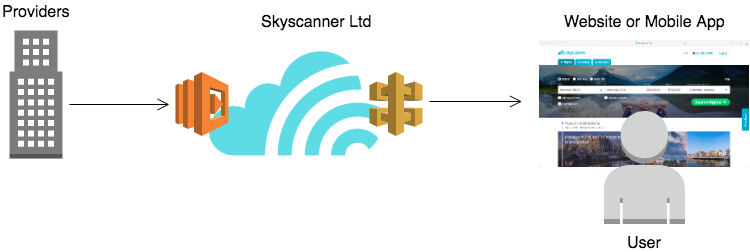
\includegraphics[scale=0.45]{diagrams/state-of-the-art-tribes-mp.png}
\caption{Simple explanation of Marketplace Engine data flow.}
\end{figure}

\subsection{Data Tribe} \label{data_tribe}

In the other hand, Data Tribe has a lot of squads with services used to collect \textbf{data from user's activity}. The flow of the information is \textit{from the user to \company}.

\begin{figure}[H]
\centering
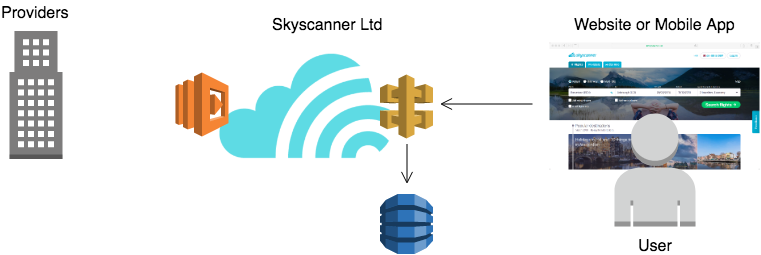
\includegraphics[scale=0.45]{diagrams/state-of-the-art-tribes-data.png}
\caption{Simple explanation of Data Tribe data flow.}
\end{figure}

\subsection{The gap}

There is no tribe or squad that works with both \textbf{data sources}: Providers and Users. And here is where the \textit{Heatmap} will be.

\begin{figure}[H]
\centering
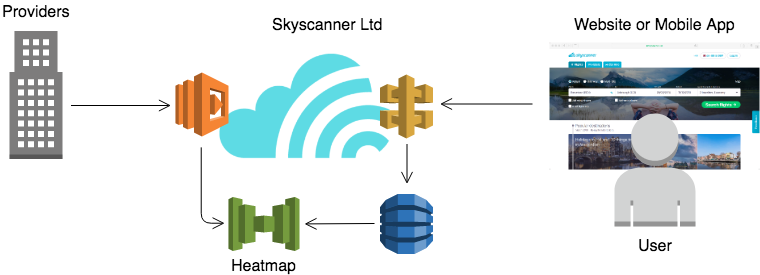
\includegraphics[scale=0.45]{diagrams/state-of-the-art-tribes-hm.png}
\caption{First approach of the Heatmap's data flow.}
\end{figure}


% Chapter 3: Scope of the project

\chapter{\company\ Heatmap}

\label{chapter03}

%-----------------
%   SECTION 3.1
%-----------------

\section{Formulation of the problem} \label{problem}

The main goal of this project is creating a tool for \textit{\company} to ease the routes and airports comparison by different parameters, taking into account values like \textbf{user demand} and \textbf{flights provided} by airlines.
\\\\
In any team of \company, user queries and providers data is compared in order to guess valuable trends.
\\\\
Found that gap, a bunch of new ideas appeared. After some talks with product owners of different squads and some senior engineers, a promising idea showed up:
\\\\
Comparison of \textbf{user demand} and \textbf{flights offered} by airlines, enabling finding \textit{over-requested} routes or airports. Those routes or airports with more user demand than offers by the providers.
\\\\
\squad\ manages a huge amount of data: All flights planned for the next two years, this are more than 75 million records. The database of all user queries in the website or mobile application is even bigger\footnote{For instance, if there were only one query per visitor the database would have 4 million new records per day}. Not much more information needed to say that this is \textbf{Big Data} problem.
\\\\
With \squad's product owner help, we found some use cases for the processing of those 75 million routes and all user session's queries to get some significant results:
\\\\
Provide a \textbf{visual tool} to find routes and airports with much \textbf{more demand than offer} and be able to observe the \textbf{evolution} of it {through time}:

\begin{itemize}
  \item A route or airport with a lot of demand, but not enough offer to cover it, will be \textbf{over-requested}.
  \item A route or airport with much more offer, but not that amount of demand, will be \textbf{non-profitable}.
\end{itemize}

%-----------------
%   SECTION 3.2
%-----------------

\section{Scope}

Merging both data sources (providers and users) generates a lot of new valuable data with a lot of different application: From simply selling it to providers, to complex deep learning systems.
\\
The final goal of this project is displaying the comparison in a simple Web UI for Marketing squads or tribes. This can be split in three smaller goals or components:

\subsection{Pipeline}

Distributed application that maps and merge all the data from both sources in its given format to the required data model.
\\\\
The pipeline reads from \nameref{mp_engine} and \nameref{data_tribe} services. Then, it maps the provider and user data to the desired data model. The new entities are stored in a database where the service will read from.
\\\\
The application will be split in two sub applications, one for providers data and other for users. So both of them can vary independently without depending on each others' sources and changes may have in the future.

\subsection{Service}

Simple HTTP Service with a basic Application Programming Interface to serve Pipeline's results. The service will have an internal endpoint only available for other \company\ applications or developers.

\subsection{Visual representation} \label{visual_representation}

Website with a visual representation of the data. There are plenty of ways to draw charts and maps visualizations. The Web UI will be composed by three main pages:

\subsubsection*{World Map}

Interactive world map with all airports represented with a dot. The radius of the dot depends on the amount of flights the airport operates.
\\\\
The Heatmap user will be able to select an airport, set a date and go to \nameref{chart_visualization} page. Another option is to select two airports, first the origin, then the destination, set a date and go to the \nameref{chart_visualization} page. If the user does not want to select the entity through the map, he/she can search it using the \nameref{browser}.

\begin{figure}[H]
\centering
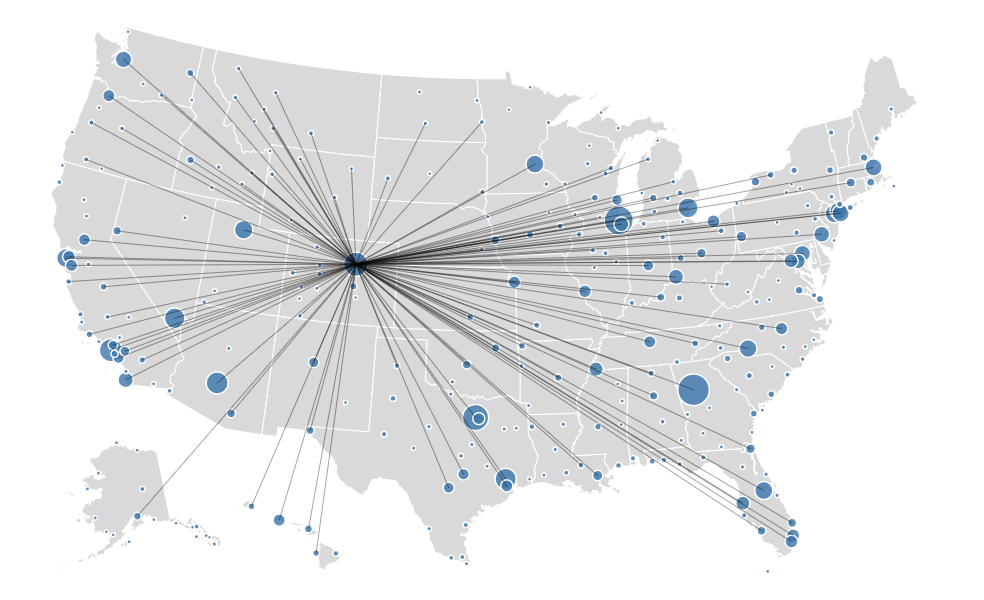
\includegraphics[scale=0.2]{resources/us-map-example01.png}
\caption{Example of the world map style. Only displaying the US to make it look clearer.}
\end{figure}

\subsubsection*{Browser} \label{browser}

Simple browser with two tabs: \textit{Route} and \textit{Airport}. In the route browser will appear three input text fields, one for the origin airport, the second for the destination and the last one for the date. In the airport browser will only appear two input text fields, airport and date.
\\\\
Once the inputs are set, the user will be able to click the \textit{Search} button and move to the next page.

\subsubsection*{Chart visualization} \label{chart_visualization}

Simple chart with the comparison between providers offer and user demand of the selected entity through time.

\begin{figure}[H]
\centering
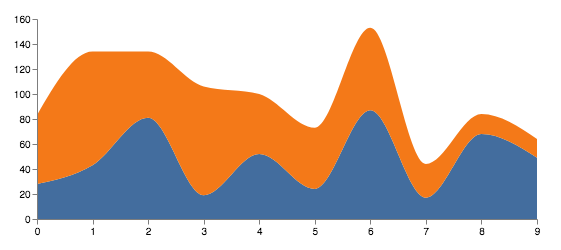
\includegraphics[scale=0.4]{resources/stacked-chart-example01.png}
\caption{Chart mock-up. One color goes for Providers Offer and the other one for User Demand.}
\end{figure}

\subsection{Not list} \label{not_list}

It is also important to define what this project will \textbf{not} be.

% WIP
\begin{itemize}
  \item \textbf{Prices} or \textbf{quotes}: In any moment will check for flight prices or quotes.
  \item \textbf{Carriers}, \textbf{cities} and \textbf{countries}: The comparison will be only available between routes and airports, not airlines (carriers), cities nor countries.
  \item \textbf{Create}, \textbf{update} or \textbf{delete} data through the \textbf{Server}: The only input will come from the pipeline. Entities are never deleted or modified in order to keep historical data.
  \item \textbf{Create}, \textbf{update} or \textbf{delete} data through the \textbf{Web UI}: The only input will come from the pipeline. Entities are never deleted or modified in order to keep historical data.
\end{itemize}

%-----------------
%   SECTION 3.3
%-----------------

\section{Risks}

There are several risks can appear while developing the project. Most risks appear because of the dependencies with other tribes and squads and dependencies with other services. In the other hand, all performance risks of the Pipeline can be ignored because \company's hardware is enough for big applications, like this one.

\subsection{Routes contract}

\squad's routes service is under development and during the Heatmap development the routes data model may change a little bit. For example, the origin and destination recently changed: In December 2017 the service was giving an \textit{Airport ID}, but now is giving an Airport object with more parameters like IATA Code\cite{iata_code}, Country ID, City ID, etc.

\subsection{Users information}

In the website and mobile application, the user have plenty of different ways to search the perfect flight. The most common one is by origin, destination and date, but he/she can also search by month or by destination. The user does not search flights for a given route in a given date. It sets the period of time he/she can travel and \company\ offers cheap destinations.
\\\\
This way of searching flights may be difficult for comparing with routes and airports offer, because sometimes the route is the actual result and not the query.

\subsection{Amount of data}

As explained before in the \nameref{problem}, there is a very big amount of data that need to be mapped. Luckily, \company\ have great cloud machines and \textit{unlimited} space\footnote{Read more in section \nameref{res_and_env}}. Anyway, still an issue to be aware of.

\subsection{Web UI}

Creating the interactive map and plots for the proposed website from zero, is a whole project itself. In order to avoid failing in the \textit{\nameref{visual_representation}} goal, the best option is to use reliable libraries, like Vega\cite{vega}.

%-----------------
%   SECTION 3.4
%-----------------

\section{Methodology and rigor} \label{methodology_rigor}

\subsection{Extreme Programming} \label{xp}

This project will be developed along with \squad's work. This squad is following Scrum, an agile methodology. After some research and discussions with the rest of the team, Extreme Programming (XP)\cite{xp} showed up as the best option.
\\\\
XP is a style of software development focused in excellent applications, programming techniques and clear communication. To accomplish that, XP includes a philosophy of software development, body of practices, complementary principles and a community that shares these values.
\\\\
This methodology works with short development cycles, resulting in early, concrete and continuing feedback. Has an incremental approach, making way to a flexible schedule for the implementation. It relies in oral communication and tests to reach the goal of the project.
\\\\
The original Extreme Programming methodology is for teams of developers, but this project will be only developed by myself, so the original idea has been modified a little bit. The pair programming and pair negotiation has been removed because I have nobody to pair with. In order to have some feedback and update the requirements properly with the supervisor, Francisco López, approval, I will be attending all \squad\ stand up meetings and explaining my progress and, if necessary, create meetings with the product owner and the rest of the squad to take the project on the right track.

\begin{figure}[H]
\centering
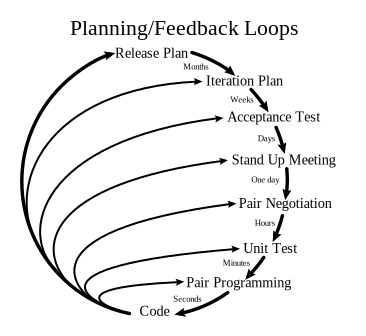
\includegraphics[scale=0.25]{diagrams/extreme_programming.png}
\caption{Extreme programming planning loops.}
\end{figure}

\subsection{GitLab}

This platform will be the main tool for version control of the source code and issue tracking of different tasks.

\subsubsection*{\texttt{git}}

All code projects (pipelines, service and website) will be stored in my personal projects space in \company's GitLab domain. Task and issue projects will be related to each project.
\\\\
Using \texttt{git}, the versions will be forked in branches, each branch will stand for an specific issue. \textit{Master} will be the main branch where the latest production version will be.

\subsubsection*{Tasks and issues}

The \textbf{issue tracking} will be very helpful in order to monitor the evolution of the project. Issues will be composed by a title, description, milestone, labels (if needed), due date and weight, and represents a new functionality. In order to know the status, issues will be listed in three columns:
\\\\
\textbf{Backlog:} Known tasks that haven been started yet. Could be a well defined task, with a very clear description, a due date and weight, or just a draft with empty fields.
\\
\textbf{WIP:} Work in Progress. The task is being considered, developed or tested.
\\
\textbf{Done:} Tasks finished, tested and working fine. Ready for production.

% Chapter 4: Requirements analysis

\chapter{Requirements analysis}

\label{chapter04}

\section{Actors}

Initially it seemed difficult to find stakeholders and actors in these project apart from the providers. It is not a tool for the user of \company\, so, as explained before, one risk of these project was not finding enough support.
\\\\
After walking with the Squad Lead and then the Product Own of \squad\ a lot of stakeholders appeared: DeLorean Squad, Marketing Automation Squad, State Machine Squad, etc. Each of these stakeholders has different use cases and the project became very interesting for a considerable part of \company\ .

\subsection{DeLorean Squad}

The mission of \squad\ is to provide the best data and services around the routes, timetables and modes of transportation to go from one point on Earth to another.
\\\\
Right now, \squad\ provides a very fast service that serves flights logistic information between a given origin and destination. Some information you can find in a route is the fight number, carriers, stops, date ranges, etc. These flights are just \textbf{single ticket flights}. The squad is currently working on more complex routes, constructed routes\footnote{Contructed Timetable contains constructed routes, routes composed by two or more single ticket flights.}.
\\\\
The constructed routes timetable is under construction, so is not available for these project. The Heatmap relies on the timetable of Single Flight Number service, also known as Timetable SFN Service.

\subsubsection{Timetable SFN Service}

The \textit{timetable SFN} endpoint returns details for time tabled Single Flight Number itineraries series. Note that SFNs are not ticket-able, so they do not include itineraries which cannot be bought on their own, neither the price nor restrictions.
\\\\
Timetable SFN Service provides all the \textbf{current} flights. This is a little bit of a problem when trying to get past routes: Timetable SFN Service does not provide past flights information, it is always \textbf{up-to-date}. In order to get this data it is needed to go one step back in the whole DeLorean data processing: Timetable Ingest Pipeline.
\\\\
Tech specifications of Timetable SFN Services are explined in section %\ref{$LABEL}.

\subsubsection{Timetable Ingest}

This phase, basically collects all the OAG\footnote{OAG file (also know as WTF file), is a CSV\cite{csv} file which each row represents a timetable for a Single Flight Number.} from a provider and maps it into routes in JSON\cite{json} format. For each different version of the OAG file, the pipeline creates a new file with all the routes.
\\\\
Then, in order to get past routes, the heatmap reference in old versions of the file created by the Timetable Ingest Pipeline.
\\\\
Tech specifications of Timetable Ingest Pipeline are explined in section %\ref{$LABEL}.

\subsection{Product Owner} \label{product_owner}

\textbf{Jen Agerton} is the Product Owner of DeLorean Squad, 

\subsection{DeLorean's Squad Lead}

\textbf{Francisco López}, who is also the supervisor of this project, and I has the initial idea for this project. He oriented it for a Machine Learning purpose.

\subsection{Neil Ross}

Neil Ross is currently the Squad Lead of \ref{marketing_atomation_squad}, this contact was given to me from my \ref{product_owner} Jen Agerton.
\\\\
After some talks through Slack\cite{slack}, he forward me extracts of the email he sent when he was in RaTS Squad, regarding to their use cases. Most of the use cases have been used for this project.

\subsubsection{Fuel RaTS Squad}

Routes and Timetable Servies Squad provides the best data and services around the routes, timetables and modes of transportation to go from one point on Earth to another. Fuel RaTS has the same mission as DeLorean Squad, but develop different services. Since Fuel RaTS provides basic routes data, pricing, live update information and multi-destination combinationcs, \squad\ provides a very fast service for only routes.

\subsubsection{Marketing Automation squad} \label{marketing_atomation_squad}

Marketing Automation squad enables scalable growth by automating workflows, and the collection of insightful data. They have three main goals:

\begin{itemize}
  \item Provide data to support decision making
  \item Automated, data driven campaign management
  \item Budget process automation
\end{itemize}

MAS provides fourteen 

\subsection{Providers}

\subsection{Competitors}

\section{Functional requirements}

\section{Non functional requirements}

\section{Use cases}

% ...
% Chapter 5: Project planning

\chapter{Project planning}

\label{chapter05}

Before defining tasks and time distribution of those, it is important to remember that this project will be developed under an Agile Methodology, \nameref{xp}. XP attempts to reduce costs of changes in requirements and long term plans, this means that this \textit{time planning} will provably change during the development. Every week a small iteration plan will be made in order to adjust the tasks with the scope and time of the project.
\\\\
Even so, here is a general plan. Tasks has been \textbf{grouped regardless the technology}, for instance: Task 27, Home Page from the Web UI. It will be developed in HyperText Markup Language and Java Script, but there is only one task for it. As explained in the previous paragraph, it is defined this way for now, in order to be agile in changes of the requirements. Then, tasks are grouped in \textbf{Milestones}.
\\\\
Milestones are used to mark specific points or goals along of a project \textit{timeline}. Milestones are very useful in order to do not losing time perception in long software projects when using Agile Methodologies, in which there are not usually to many deadlines.
\\\\
Another important thing to take into account is the \textbf{tasks overlapping}. Is a good practice\cite{clean_coder} not to work to much time in the same thing, task or goal. Swapping between different tasks and milestones can help so the developer \textbf{does not obfuscate}.
\\\\
Last but not least, there are two holiday weeks in March, one is \textit{Holy week} (13th), and the other is extra. That is why the project starts earlier.

%-----------------
%   SECTION 5.1
%-----------------

\section{Tasks}

Development tasks (from 14 to 30) duration is specified in days. Weeks are composed by five working days, so 5 days equals to a week. In a day, the developer is supposed to work five hours. From week seven to week twenty-three, there are fifteen working weeks (not counting holidays). Doing simple maths, the development will take:
\\
$$15\ \textrm{weeks} \times 5\ \frac{\textrm{days}}{\textrm{week}} \times 5\ \frac{\textrm{hours}}{\textrm{day}} = 375\ \textrm{hours}$$
\\
\textbf{375 hours} of development.
\\\\
It is important to understand that similar tasks like 16th and 20th or 17th and 21st have different times, that is because the second time it is supposed to be very similar than the first, so there will be some previous knowledge when executing it for second time.

%-------------------
%   SECTION 5.1.1
%-------------------

\subsection{Inception}

Regard this an agile project, there has been an small inception part where the project was predefined and explained to \company\ product owners to see if it was viable.

\begin{table}[H]
\begin{tabular}{>{\raggedleft\arraybackslash}p{3cm}>{\raggedright\arraybackslash}p{11cm}}
\textbf{Name}        & Inception \\
\textbf{Number}      & 1 \\
\textbf{Description} & Identify the initial scope of the project, stakeholders, context and environment where the project will be developed. \\
\textbf{End date}    & 9th of February, 2018 \\
\end{tabular}
\label{milestone1}
\end{table}

\begin{table}[H]
\begin{tabular}{>{\raggedleft\arraybackslash}p{3cm}>{\raggedright\arraybackslash}p{11cm}}
\textbf{Name}        & Definition of the problem \\
\textbf{Number}      & 2 \\
\textbf{Description} & Defining, at a high level, what the system will do. \\
\textbf{Duration}    & 10 days \\
\textbf{Milestone}   & \nameref{milestone1} \\
\textbf{Dependencies}& -- \\
\end{tabular}
\end{table}

\begin{table}[H]
\begin{tabular}{>{\raggedleft\arraybackslash}p{3cm}>{\raggedright\arraybackslash}p{11cm}}
\textbf{Name}        & Scope \\
\textbf{Number}      & 3 \\
\textbf{Description} & What the software project will do and will not. Not list. \\
\textbf{Duration}    & 5 days \\
\textbf{Milestone}   & \nameref{milestone1} \\
\textbf{Dependencies}& 2: Definition of the problem \\
\end{tabular}
\end{table}

\begin{table}[H]
\begin{tabular}{>{\raggedleft\arraybackslash}p{3cm}>{\raggedright\arraybackslash}p{11cm}}
\textbf{Name}        & Risks \\
\textbf{Number}      & 4 \\
\textbf{Description} & Find possible problems and obstacles may appear in the future development. \\
\textbf{Duration}    & 8 days \\
\textbf{Milestone}   & \nameref{milestone1} \\
\textbf{Dependencies}& 3: Scope \\
\end{tabular}
\end{table}

\begin{table}[H]
\begin{tabular}{>{\raggedleft\arraybackslash}p{3cm}>{\raggedright\arraybackslash}p{11cm}}
\textbf{Name}        & Scope refinement \\
\textbf{Number}      & 5 \\
\textbf{Description} & After finding the risks, review the scope. Make it possible. \\
\textbf{Duration}    & 4 days \\
\textbf{Milestone}   & \nameref{milestone1} \\
\textbf{Dependencies}& 4: Risks \\
\end{tabular}
\end{table}

\begin{table}[H]
\begin{tabular}{>{\raggedleft\arraybackslash}p{3cm}>{\raggedright\arraybackslash}p{11cm}}
\textbf{Name}        & Environment \\
\textbf{Number}      & 6 \\
\textbf{Description} & Find the correct environment in order to build the project. \\
\textbf{Duration}    & 2 days \\
\textbf{Milestone}   & \nameref{milestone1} \\
\textbf{Dependencies}& 5: Scope refinement \\
\end{tabular}
\end{table}

%-------------------
%   SECTION 5.1.2
%-------------------

\subsection{Project management}

\begin{table}[H]
\begin{tabular}{>{\raggedleft\arraybackslash}p{3cm}>{\raggedright\arraybackslash}p{11cm}}
\textbf{Name}        & Project management (GEP) \\
\textbf{Number}      & 7 \\
\textbf{Description} & First stage in the TFG. Get thesis started. \\
\textbf{End date}    & 20th of April, 2018 \\
\end{tabular}
\label{milestone2}
\end{table}

\begin{table}[H]
\begin{tabular}{>{\raggedleft\arraybackslash}p{3cm}>{\raggedright\arraybackslash}p{11cm}}
\textbf{Name}        & Context and scope \\
\textbf{Number}      & 8 \\
\textbf{Description} & Indicate general objective of the TFG and context. \\
\textbf{Duration}    & 12 days \\
\textbf{Milestone}   & \nameref{milestone2} \\
\textbf{Dependencies}& -- \\
\end{tabular}
\label{deliverable1}
\end{table}

\begin{table}[H]
\begin{tabular}{>{\raggedleft\arraybackslash}p{3cm}>{\raggedright\arraybackslash}p{11cm}}
\textbf{Name}        & Project planning \\
\textbf{Number}      & 9 \\
\textbf{Description} & Planning of the entire execution of the TFG. \\
\textbf{Duration}    & 4 days \\
\textbf{Milestone}   & \nameref{milestone2} \\
\textbf{Dependencies}& 8: Context and scope \\
\end{tabular}
\label{deliverable2}
\end{table}

\begin{table}[H]
\begin{tabular}{>{\raggedleft\arraybackslash}p{3cm}>{\raggedright\arraybackslash}p{11cm}}
\textbf{Name}        & Budget and sustainability \\
\textbf{Number}      & 10 \\
\textbf{Description} & Explanation of the sustainability of the project. Economical, social and environmental. \\
\textbf{Duration}    & 5 days \\
\textbf{Milestone}   & \nameref{milestone2} \\
\textbf{Dependencies}& 9: Project planning \\
\end{tabular}
\label{deliverable3}
\end{table}

\begin{table}[H]
\begin{tabular}{>{\raggedleft\arraybackslash}p{3cm}>{\raggedright\arraybackslash}p{11cm}}
\textbf{Name}        & First oral presentation \\
\textbf{Number}      & 11 \\
\textbf{Description} & Three minute oral presentation on video. \\
\textbf{Duration}    & 10 days \\
\textbf{Milestone}   & \nameref{milestone2} \\
\textbf{Dependencies}& 10: Budget and sustainability \\
\end{tabular}
\end{table}

\begin{table}[H]
\begin{tabular}{>{\raggedleft\arraybackslash}p{3cm}>{\raggedright\arraybackslash}p{11cm}}
\textbf{Name}        & Competences review \\
\textbf{Number}      & 12 \\
\textbf{Description} & Review of the competences of the bachelor's thesis. \\
\textbf{Duration}    & 5 days \\
\textbf{Milestone}   & \nameref{milestone2} \\
\textbf{Dependencies}& -- \\
\end{tabular}
\end{table}

\begin{table}[H]
\begin{tabular}{>{\raggedleft\arraybackslash}p{3cm}>{\raggedright\arraybackslash}p{11cm}}
\textbf{Name}        & Final document \\
\textbf{Number}      & 13 \\
\textbf{Description} & \nameref{deliverable1}, \nameref{deliverable2} and \nameref{deliverable3}. Reviewed. \\
\textbf{Duration}    & 5 days \\
\textbf{Milestone}   & \nameref{milestone2} \\
\textbf{Dependencies}& 11: First oral presentation \\
\end{tabular}
\end{table}

%-------------------
%   SECTION 5.1.3
%-------------------

\subsection{Flights offer pipeline}

\begin{table}[H]
\begin{tabular}{>{\raggedleft\arraybackslash}p{3cm}>{\raggedright\arraybackslash}p{11cm}}
\textbf{Name}        & Flights offer pipeline \\
\textbf{Number}      & 14 \\
\textbf{Description} & Application that maps the provider data to the desired data model. \\
\textbf{End date}    & 16th of March, 2018 \\
\end{tabular}
\label{milestone3}
\end{table}

\begin{table}[H]
\begin{tabular}{>{\raggedleft\arraybackslash}p{3cm}>{\raggedright\arraybackslash}p{11cm}}
\textbf{Name}        & Reading from DeLorean's pipeline \\
\textbf{Number}      & 15 \\
\textbf{Description} & Connect to DeLorean's application that gets all routes and read from it \\
\textbf{Duration}    & 5 days \\
\textbf{Milestone}   & \nameref{milestone3} \\
\textbf{Dependencies}& -- \\
\end{tabular}
\end{table}

\begin{table}[H]
\begin{tabular}{>{\raggedleft\arraybackslash}p{3cm}>{\raggedright\arraybackslash}p{11cm}}
\textbf{Name}        & Data processing \\
\textbf{Number}      & 16 \\
\textbf{Description} & Filter and map all data in DeLorean's model to desired for the \thesistitle. \\
\textbf{Duration}    & 10 days \\
\textbf{Milestone}   & \nameref{milestone3} \\
\textbf{Dependencies}& 15: Reading from DeLorean's pipeline \\
\end{tabular}
\end{table}

\begin{table}[H]
\begin{tabular}{>{\raggedleft\arraybackslash}p{3cm}>{\raggedright\arraybackslash}p{11cm}}
\textbf{Name}        & Writing into service DB \\
\textbf{Number}      & 17 \\
\textbf{Description} & Once the data is processed, write into the service DB \\
\textbf{Duration}    & 10 days \\
\textbf{Milestone}   & \nameref{milestone3} \\
\textbf{Dependencies}& 16: Data processing \\
\end{tabular}
\end{table}

%-------------------
%   SECTION 5.1.4
%-------------------

\subsection{User searches pipeline}

\begin{table}[H]
\begin{tabular}{>{\raggedleft\arraybackslash}p{3cm}>{\raggedright\arraybackslash}p{11cm}}
\textbf{Name}        & User searches pipeline \\
\textbf{Number}      & 18 \\
\textbf{Description} & Application that maps the user data to the desired data model. \\
\textbf{End date}    & 27th of April, 2018 \\
\end{tabular}
\label{milestone4}
\end{table}

\begin{table}[H]
\begin{tabular}{>{\raggedleft\arraybackslash}p{3cm}>{\raggedright\arraybackslash}p{11cm}}
\textbf{Name}        & Reading from Data Tribe BD \\
\textbf{Number}      & 19 \\
\textbf{Description} & Find correct table and read from Data Tribe DB service. \\
\textbf{Duration}    & 10 days \\
\textbf{Milestone}   & \nameref{milestone4} \\
\textbf{Dependencies}& -- \\
\end{tabular}
\end{table}

\begin{table}[H]
\begin{tabular}{>{\raggedleft\arraybackslash}p{3cm}>{\raggedright\arraybackslash}p{11cm}}
\textbf{Name}        & Data processing \\
\textbf{Number}      & 20 \\
\textbf{Description} & Filter and map all data in Data Tribe's model to desired for the \thesistitle. \\
\textbf{Duration}    & 5 days \\
\textbf{Milestone}   & \nameref{milestone4} \\
\textbf{Dependencies}& 19: Reading from Data Tribe BD \\
\end{tabular}
\end{table}

\begin{table}[H]
\begin{tabular}{>{\raggedleft\arraybackslash}p{3cm}>{\raggedright\arraybackslash}p{11cm}}
\textbf{Name}        & Writing into service DB \\
\textbf{Number}      & 21 \\
\textbf{Description} & Once the data is processed, write into the service DB \\
\textbf{Duration}    & 5 days \\
\textbf{Milestone}   & \nameref{milestone4} \\
\textbf{Dependencies}& 20: Data processing \\
\end{tabular}
\end{table}

%-------------------
%   SECTION 5.1.5
%-------------------

\subsection{Heatmap server}

\begin{table}[H]
\begin{tabular}{>{\raggedleft\arraybackslash}p{3cm}>{\raggedright\arraybackslash}p{11cm}}
\textbf{Name}        & Heatmap server \\
\textbf{Number}      & 22 \\
\textbf{Description} & Web server that provides all data processed by pipelines \\
\textbf{End date}    & 19th of May, 2018 \\
\end{tabular}
\label{milestone5}
\end{table}

\begin{table}[H]
\begin{tabular}{>{\raggedleft\arraybackslash}p{3cm}>{\raggedright\arraybackslash}p{11cm}}
\textbf{Name}        & Reading offer \\
\textbf{Number}      & 23 \\
\textbf{Description} & Read offer from DB, wrote by \nameref{milestone3} \\
\textbf{Duration}    & 5 days \\
\textbf{Milestone}   & \nameref{milestone5} \\
\textbf{Dependencies}& 17: Writing into service DB \\
\end{tabular}
\end{table}

\begin{table}[H]
\begin{tabular}{>{\raggedleft\arraybackslash}p{3cm}>{\raggedright\arraybackslash}p{11cm}}
\textbf{Name}        & Reading demand \\
\textbf{Number}      & 24 \\
\textbf{Description} & Read offer from DB, wrote by \nameref{milestone4} \\
\textbf{Duration}    & 5 days \\
\textbf{Milestone}   & \nameref{milestone5} \\
\textbf{Dependencies}& 20: Writing into service DB \\
\end{tabular}
\end{table}

\begin{table}[H]
\begin{tabular}{>{\raggedleft\arraybackslash}p{3cm}>{\raggedright\arraybackslash}p{11cm}}
\textbf{Name}        & Comparison \\
\textbf{Number}      & 25 \\
\textbf{Description} & Provide comparison of both sources. \\
\textbf{Duration}    & 10 days \\
\textbf{Milestone}   & \nameref{milestone5} \\
\textbf{Dependencies}& 23: Reading offer, 24: Reading demand \\
\end{tabular}
\end{table}

%-------------------
%   SECTION 5.1.6
%-------------------

\subsection{Heatmap Web UI}

\begin{table}[H]
\begin{tabular}{>{\raggedleft\arraybackslash}p{3cm}>{\raggedright\arraybackslash}p{11cm}}
\textbf{Name}        & Heatmap Web UI \\
\textbf{Number}      & 26 \\
\textbf{Description} & Website with a visual representation of the data. \\
\textbf{End date}    & 8th of June, 2018 \\
\end{tabular}
\label{milestone6}
\end{table}

\begin{table}[H]
\begin{tabular}{>{\raggedleft\arraybackslash}p{3cm}>{\raggedright\arraybackslash}p{11cm}}
\textbf{Name}        & Home page \\
\textbf{Number}      & 27 \\
\textbf{Description} & World map with all airports, just geographical localization. \\
\textbf{Duration}    & 5 days \\
\textbf{Milestone}   & \nameref{milestone6} \\
\textbf{Dependencies}& -- \\
\end{tabular}
\end{table}

\begin{table}[H]
\begin{tabular}{>{\raggedleft\arraybackslash}p{3cm}>{\raggedright\arraybackslash}p{11cm}}
\textbf{Name}        & Search page \\
\textbf{Number}      & 28 \\
\textbf{Description} & Search inputs for querying the service. \\
\textbf{Duration}    & 5 days \\
\textbf{Milestone}   & \nameref{milestone6} \\
\textbf{Dependencies}& -- \\
\end{tabular}
\end{table}

\begin{table}[H]
\begin{tabular}{>{\raggedleft\arraybackslash}p{3cm}>{\raggedright\arraybackslash}p{11cm}}
\textbf{Name}        & Data representation \\
\textbf{Number}      & 29 \\
\textbf{Description} & Get data from service and display it in the views. \\
\textbf{Duration}    & 10 days \\
\textbf{Milestone}   & \nameref{milestone6} \\
\textbf{Dependencies}& 25: Comparison, 27: Home page, 28: Search page \\
\end{tabular}
\end{table}

\begin{table}[H]
\begin{tabular}{>{\raggedleft\arraybackslash}p{3cm}>{\raggedright\arraybackslash}p{11cm}}
\textbf{Name}        & Chart view \\
\textbf{Number}      & 30 \\
\textbf{Description} & Chart showing the route or airport comparison. \\
\textbf{Duration}    & 5 days \\
\textbf{Milestone}   & \nameref{milestone6} \\
\textbf{Dependencies}& 29: Data representation \\
\end{tabular}
\end{table}

%-------------------
%   SECTION 5.1.7
%-------------------

\subsection{Final presentation}

\begin{table}[H]
\begin{tabular}{>{\raggedleft\arraybackslash}p{3cm}>{\raggedright\arraybackslash}p{11cm}}
\textbf{Name}        & Final presentation \\
\textbf{Number}      & 31 \\
\textbf{Description} & TFG whole report document and prepare the final presentation. \\
\textbf{End date}    & 22nd of June, 2018 \\
\end{tabular}
\label{milestone7}
\end{table}

%-----------------
%   SECTION 5.2
%-----------------

\section{Alternatives}

In case the project takes too much time, both pipelines can be totally overlapped. This will reduce the number of weeks from fifteen to eleven.
\\\\
Another option is to remove the some pipeline, the server will provably have a higher latency, but it will reduce to ten or eleven weeks. 

%-----------------
%   SECTION 5.3
%-----------------

\section{Gantt}

\begin{figure}[p]
\centering
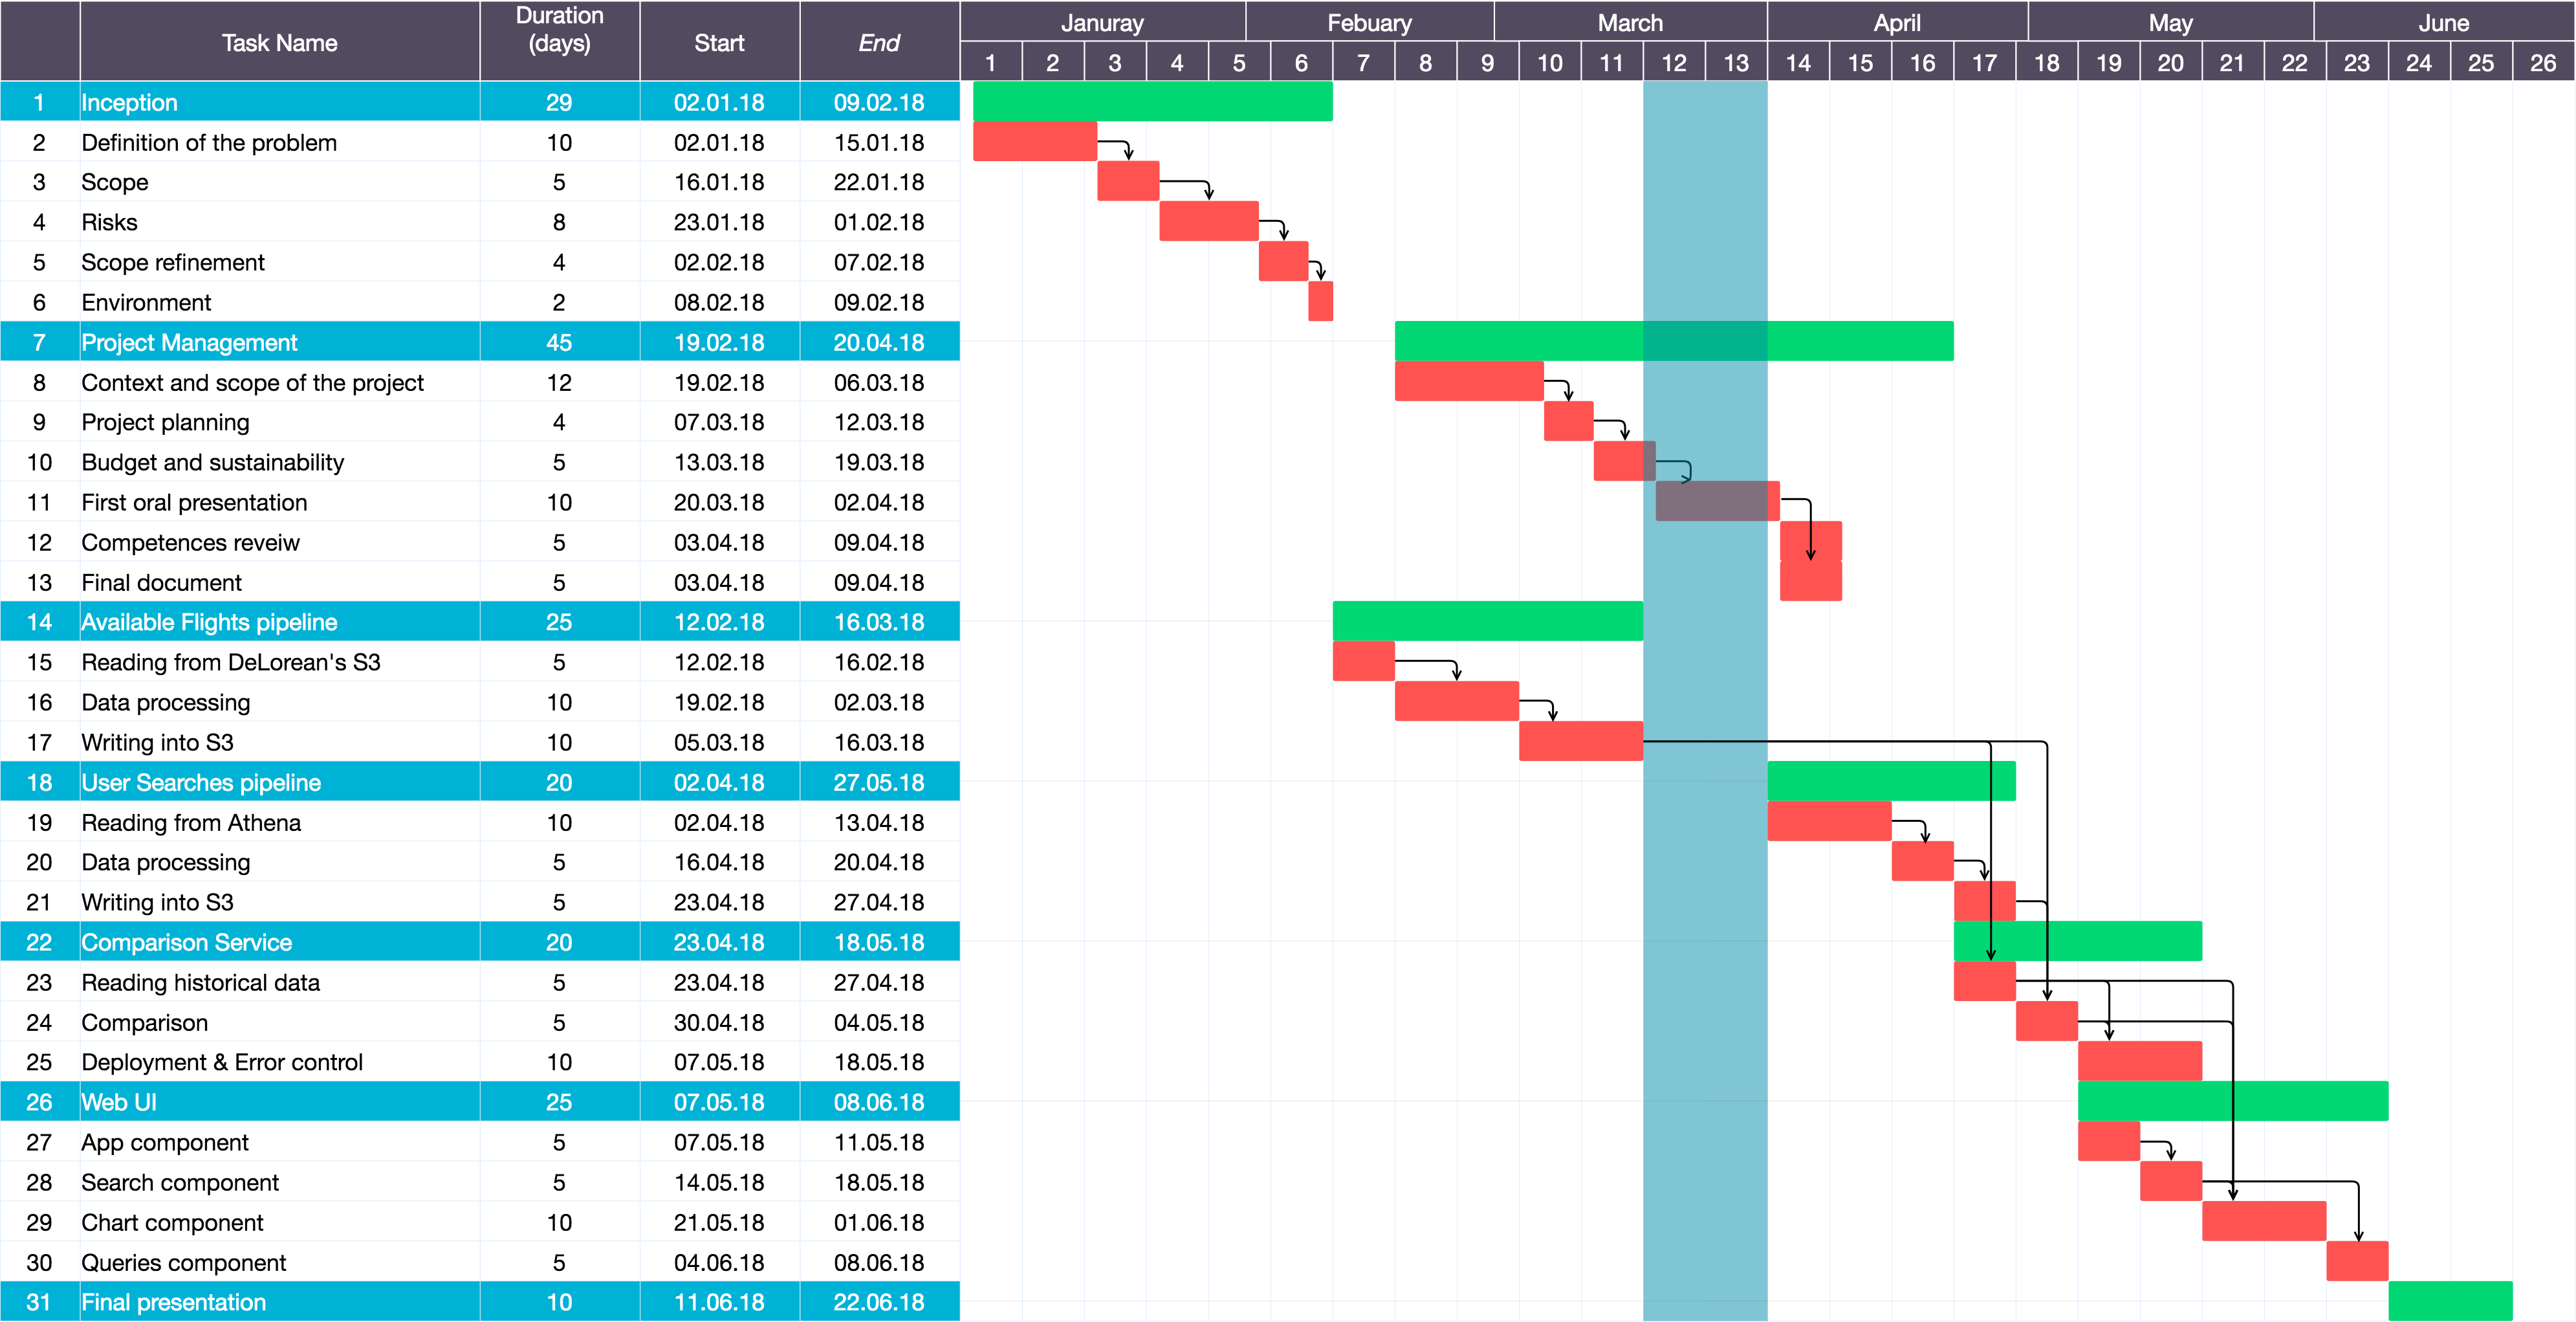
\includegraphics[scale=0.175,  angle =90]{diagrams/gantt.png}
\caption{Gantt diagram.}
\end{figure}




% Chapter 6: Budget and sustainability

\chapter{Budget and Sustainability}

\label{chapter06}

\section{Budget}

Once the project is planned in time and its technologies are drafted, we can calculate the project’s budget.
Skyscanner is not economically transparent, even for the employees. So, this whole calculation will be approximated.
\\\\
First of all, we have to take into account the employees, which is only one and in Intern position, and also count the taxes.
\\\\
Apart from that, all the hardware material and software licenses. AWS costs will continue but since it is going to be used during the development for testing it is counted in the total budget.

\begin{table}[H]
\centering
\begin{tabular}{|l|l|l|l|l|}
\hline
\textbf{Concept}           & \textbf{Price per unit} & \textbf{Units} & \textbf{Amortization} & \textbf{Total £}   \\ \hline
\textbf{Salary}            & 28 (taxes included)     & 575 h          &                       & 16100              \\ \hline
\textbf{MacBook Pro}       & 1700                    & 1              & life cycle 8 years    & 210                \\ \hline
\textbf{JetBrains License} & 230                     & 1              & 1 year per developer  & 130                \\ \hline
\textbf{AWS S3}            & 0.023                   & 50 TB          &                       & 1150               \\ \hline
\textbf{AWS}               & EC2                     & 575 h          &                       & 213.325            \\ \hline
\textbf{Screen}            & 200                     & 2              & life cycle 4 years    & 100                \\ \hline
\textbf{Office}            & Uknown                  & 1              &                       & Uknown             \\ \hline
\textbf{TOTAL}             &                         &                &                       & \textbf{17903.325} \\ \hline
\end{tabular}
\caption{Budget calculation}
\label{budget-calculation}
\end{table}

\section{Sustainability}

\subsection{Economical}

In economic terms, this project is initially unsustainable. It uses resources from Skyscanner for a comparison that might be useful in the future for other projects, improving some services or advertisement.
\\\\
But, if this product is sell to providers, Skyscanner can take a lot of profit from them. It is a very valuable application for providers, since they could compare airlines offer with actual user demand. Letting them improve their flights distribution and make more money.

\subsection{Social}

The \thesistitle is not directly involving society, but, as explained before, if providers have access to the comparison, flights will improve in terms of traveler experience. Travelers will have accurate routes depending on what they really want.
\\\\
For example, imagine that X carrier have several flights from BCN to ORY, Paris, and a few from BCN to FCO, Rome. The \thesistitle shows that the demand, compared with the offer is bigger in Rome than in Paris. Then, X airline could schedule more flights to FCO instead of ORY.

\subsection{Environment}

The environmental impact of the \thesistitle is directly related with the social impact.
\\\\
Right now, some airlines may have half full flights. This means that the airplane is not taking its most advantage of the fuel. It could be carrying more people.
\\\\
If carriers know where flights are really needed those flight will be full of people, which means that the fuel a flight uses is profited at its most.
\\\\
Otherwise, if an offer is under requested, the flight is not giving all the profit it could.
In other words, fuel per person will decrease.

\subsection{Sustainability matrix}

In order to understand the general impact of the project, the following general rating and evaluation is provided:
\\\\
The economical impact will be rated in 7/10. It could be a 10/10 it is sell to providers. Air companies could pay a lot of money for the \thesistitle because of the information it provides.
\\\\
The social impact will get a 4/10. It does nothing good nor bad to the society, only if the application is sell to providers and they use it properly, it could make some good to the people. In the other hand, the software will not be free, it will be property of \company.
\\\\
The environmental impact is a 4/10 as well. The environmental impact could be good if the application is sell to providers and they use it properly, but for now will not be sell to anyone. It gets a 4 because it will be using Amazon Web Service, and those machines are powered mainly by non-renewable energy\cite{click_clean}.
\\\\

\begin{table}[H]
\centering
\begin{tabular}{|l|l|l|}
\hline
Economical & Social & Environmental \\ \hline
7/10       & 4/10   & 4/10          \\ \hline
\multicolumn{3}{|l|}{15/30}         \\ \hline
\end{tabular}
\caption{Sustainability matrix}
\label{sustainability-matrix}
\end{table}


%------------------------
% CHAPTER 7: Development
%------------------------

\chapter{Development}

\label{chapter07}

Once the system is designed and its architecture defined, the implementation took an important part of the time. The \thesis\ used a lot of frameworks and libraries that eased the development. Some of them has been already explained, like \nameref{apache_spark} that offers an API to process big data dumps and it parallelizes the process automatically.
\\\\
First of all, lets check the main programming languages used in this project and then all libraries and frameworks component by component, finally the tools used for the development and deployment.

\section{Programming languages}

\subsection*{Scala\cite{scala}} \label{scala}

\begin{figure}[H]
\centering

\includegraphics[scale=0.1]{resources/scala-logo.png}
\caption{Scala logo}
\end{figure}

Scala (\texttt{.scala} as file extension) is multi-paradigm programming language compiled by the Java Virtual Machine\cite{jvm}. Its main paradigms are \textbf{functional} (very useful for \nameref{apache_spark}, Java\cite{java} also provides this since version 8, but in Scala it is much easier to write and debug) object-oriented, imperative and concurrent.
\\\\
Scala is the preferred language by the Apache Software Foundation for \nameref{apache_spark}, that is why it is the main language used in both pipelines, \nameref{available-flights-pipeline} and \nameref{user-searches-pipeline}. The latest \nameref{apache_spark} API is for Scala, then it usually comes out for Java and finally for Python.
\\\\
I have never programmed in Scala before this project, but it was very fast and easy to learn. Knowing Java, the syntax is not much different and, usually, more intuitive.

\subsection*{Python\cite{python}}

\begin{figure}[H]
\centering

\includegraphics[scale=0.1]{resources/python-logo.png}
\caption{Python logo}
\end{figure}

Python (with file extension \texttt{.py}) is the language used for the service. Python 3.6 is the version used instead of 2.7, which is very different. Python2.7 will not have support anymore in a few months.
\\\\
The syntax of python is different than C based languages and allows a lot of \textit{tricks} that the developer cannot do in most programming languages, for instance: \texttt{a[-1]} gets the last element of the array \texttt{a}. It is the only language used in the \nameref{comparison_service}, thanks to Python's flexibility; imperative, functional, object-oriented, procedure and reflective paradigms; duck, string and dynamic typing and compatibility with lost of technologies makes the service easy to be implemented in few lines.

\subsection*{JavaScript\cite{js}}

Often abbreviated as JS, JavaScript is an interpreted programming language core of the World Wide Web technologies all along with HTML\cite{html} and CSS\cite{css}. It is used in the \nameref{web-ui} and, like Python, it has compatibility with a lot of technologies, \nameref{axios}, \nameref{reactjs} and \nameref{vega}.

\begin{figure}[H]
\centering

\includegraphics[scale=0.1]{resources/www-tech-logos.jpeg}
\caption{HTML, JS and CSS logos}
\end{figure}

\section{External libraries and frameworks}

\subsection*{Scala Amazon Web Service's Software Development Kit\cite{scala_aws}} \label{scala_aws}

Amazon provides a lot of APIs for different programming languages. The AWS SDK for Java enable Java developers to easily work with Amazon Web Services and build scalable solutions with Amazon S3, Amazon Athena, Amazon DynamoDB, and more. Since Scala is assembled by the Java Virtual Machine, Amazon created the Scala Amazon Web Services SDK, it's like the AWS SDK for Java, but more Scala-y.
\\\\
Thanks to that Software Development Kit both pipelines can write to the \nameref{s3} and query \nameref{athena} in the case of the User Searches Pipeline.

\subsection*{Gson\cite{gson}} \label{gson}

Most data is usually serialized in JSON\cite{json} format, to deserialize it and get an Scala object, the Available Flights Pipeline uses Google's library Gson.

\subsection*{Boto3\cite{boto3}} \label{boto3}

This Python library is also very important for the project. It is the Amazon Web Service's Software Development Kit for Python. It is not as complete as the Java AWS SDK or the Scala AWS SDK but the \nameref{s3} API it provides is more than enough for the Comparison Service.

\subsection*{aiohttp\cite{aiohttp}} \label{aiohttp}

In order to have an Asynchronous HTTP Client and Service for Python, the \thesis\ is using AIOHTTP. One of its key features is the support to Server WebSockets.

\subsection*{axios\cite{axios}} \label{axios}

For the \nameref{web-ui} to call the \nameref{comparison_service}, axios is a JavaScript library that provides a promise based HTTP client for the browser.

\subsection*{React.js\cite{reactjs}} \label{reactjs}

React is a set of libraries combined in a single framework for building user interfaces in JavaScript. Allows the developer create a Declarative and Component-Based interface. React is build a way that when a change happens it does not render all the page again, it only renders the component that has changed, making the website much faster than typical static pages.

\subsection*{Vega\cite{vega}} \label{vega}

Interactive Data Lab created Vega and Vega Lite, a library that allows create visualization designs using a declarative format. All visualizations are described in JSON\cite{json} and Vega does all the work for you. The \nameref{web-ui} uses the Line Chart provided by Vega Lite.

\begin{figure}[H]
\centering
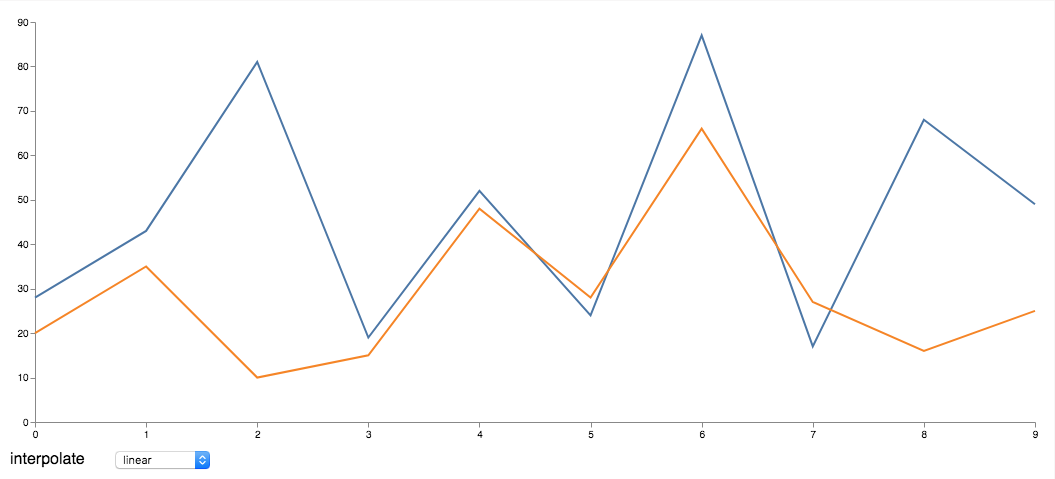
\includegraphics[scale=0.4]{resources/lineal-chart-example01.png}
\caption{Vega Lite line chart example.}
\end{figure}

\section{Developing tools}

The two main tools used for the development of the \thesis\ are IntelliJ IDEA by JetBrains and Sublime Text 3.

\subsection*{IntelliJ IDEA by JetBrains\cite{intellij}}

\begin{figure}[H]
\centering

\includegraphics[scale=0.1]{resources/intellij-logo.png}
\caption{IntelliJ IDEA logo}
\end{figure}

\textit{Capable and Ergonomic IDE for JVM}. IntelliJ is the preferred IDE\cite{ide} in \company. Ease the development of Java projects and, with a Scala Building Tool plugin IntelliJ eases the development of Scala projects. This Integrated Development Environment has been used for writing, testing, executing and assembling \nameref{available-flights-pipeline} and \nameref{user-searches-pipeline} projects.

\subsection*{Sublime Text 3\cite{sublimetext}}

\begin{figure}[H]
\centering

\includegraphics[scale=0.1]{resources/sublime-logo.png}
\caption{Sublime Text 3 logo}
\end{figure}

Sublime Text is not an IDE, is just a text editor for code, markup and prose. Sophisticated and full of features for the developers, makes easier the development of software, systems and applications that do not have an specific IDE or that the existing development environment complicates the project. That is why Sublime Text 3 has been used for the \nameref{comparison_service} and the \nameref{web-ui}.

\section{Deployment}

The deployment of the software was automatic when the new code was pushed to its \texttt{git} branch. Deployed to sandbox if the branch was a feature branch, deployed to prod if the branch was \texttt{master}.
\\\\
This process was automatic thanks to Drone. This tool can deploy to Amazon Web Service if there is an stack available created by the Amazon CloudFormation. In order to track the deployment and scheduled executions of the pipelines, the project have \nameref{sns} configured.

\subsection*{Drone}

\begin{figure}[H]
\centering

\includegraphics[scale=0.1]{resources/drone-logo.png}
\caption{Drone logo}
\end{figure}

Drone\cite{drone} is an open source Continuous Delivery platform that automates your testing and release workflows. Every repository has a \texttt{.drone.yml} file where the release workflow is described. The GitLab repository is linked with Drone and when the code is pushed Drone automatically runs the commands set for that specific \texttt{git} action.

\subsection*{Amazon CloudFormation}

\begin{figure}[H]
\centering

\includegraphics[scale=0.1]{resources/cf-logo.png}
\caption{Amazon CloudFormation logo}
\end{figure}


\subsection*{Amazon Simple Notification Service} \label{sns}

\begin{figure}[H]
\centering

\includegraphics[scale=0.1]{resources/sns-logo.png}
\caption{Amazon Simple Notification Service logo}
\end{figure}






%------------------------------
% CHAPTER 8: System evaluation
%------------------------------

\chapter{System evaluation}

\label{chapter08}
% Chapter 9: Project planning

\chapter{Project planning}

\label{chapter09}

Before defining tasks and time distribution of those, it is important to remember that this project is developed under an Agile Methodology, \nameref{xp}. XP attempts to reduce costs of changes in requirements and long term plans, this means that this \textit{time planning} is just an initial aproximation and has changed during the development. Every week a small iteration plan has been made in order to adjust the tasks with the scope and time of the project.
\\\\
Even so, here is a general plan. Tasks has been \textbf{grouped regardless the technology}, for instance\cite{w3_templates}: Task 27, App Component from the Web UI. It will have an HyperText Markup Language part only for the view and a Java Script part for getting and displaying server's data, but there is only one task for it.
\\\\
Tasks are grouped in \textbf{Milestone}. Used to mark specific points or goals along of a project timeline. Milestone are very useful in order to do not losing time perception in long software projects when using Agile Methodologies.
\\\\
Another important thing to take into account is the \textbf{tasks overlapping}. Is a good practice\cite{clean_coder} not to work to much time in the same thing, task or goal. Swapping between different tasks and milestone can help the developer to \textbf{not obfuscate}.

%-----------------
%   SECTION 9.1
%-----------------

\section{Tasks}

All development tasks (from number 14 to 30), are composed by small cycles where the developer designs, codes, tests, refactors and deploys the software. In every task the developer loops through these cycles, as explained in \nameref{methodology_rigor} section.
\\\\
Development tasks duration is specified in days. Weeks are composed by five working days, so 5 days equals to a week. In a day, the developer is supposed to work five hours. From week seven to week twenty-three, there are fifteen working weeks (not counting holidays\footnote{There are two holiday weeks in March, one is \textit{Holy week} (13th), and the other is extra. That is why the project starts earlier.}). Doing simple maths, the development will take:
\\
$$15\ \textrm{weeks} \times 5\ \frac{\textrm{days}}{\textrm{week}} \times 5\ \frac{\textrm{hours}}{\textrm{day}} = 375\ \textrm{hours}$$
\\
\textbf{375 hours} of development. Adding the small inception of the beginning and the project report in the end, 8 weeks, The whole project will take a total of \textbf{575 hours}.
\\\\
It is important to understand that similar tasks like 16th and 20th or 17th and 21st have different times, that is because the second time it is supposed to be very similar than the first, so there will be some previous knowledge when executing them for second time.

%-------------------
%   SECTION 9.1.1
%-------------------

\subsection{Inception}

Regard this an agile project, there has been an small inception part where the project was predefined and explained to \company\ product owners to see if it was viable.

\begin{table}[H]
\begin{tabular}{>{\raggedleft\arraybackslash}p{3cm}>{\raggedright\arraybackslash}p{11cm}}
\textbf{Milestone name} & Inception \\
\textbf{Number}      & 1 \\
\textbf{Description} & Identify the initial scope of the project, stakeholders, context and environment where the project will be developed. \\
\textbf{End date}    & 9th of February, 2018 \\
\end{tabular}
\label{milestone1}
\end{table}

\begin{table}[H]
\begin{tabular}{>{\raggedleft\arraybackslash}p{3cm}>{\raggedright\arraybackslash}p{11cm}}
\textbf{Name}        & Definition of the problem \\
\textbf{Number}      & 2 \\
\textbf{Description} & Defining, at a high level, what the system will do. \\
\textbf{Duration}    & 10 days \\
\textbf{Milestone}   & \nameref{milestone1} \\
\textbf{Dependencies}& -- \\
\end{tabular}
\end{table}

\begin{table}[H]
\begin{tabular}{>{\raggedleft\arraybackslash}p{3cm}>{\raggedright\arraybackslash}p{11cm}}
\textbf{Name}        & Scope \\
\textbf{Number}      & 3 \\
\textbf{Description} & What the software project will do and will not. Not list. \\
\textbf{Duration}    & 5 days \\
\textbf{Milestone}   & \nameref{milestone1} \\
\textbf{Dependencies}& 2: Definition of the problem \\
\end{tabular}
\end{table}

\begin{table}[H]
\begin{tabular}{>{\raggedleft\arraybackslash}p{3cm}>{\raggedright\arraybackslash}p{11cm}}
\textbf{Name}        & Risks \\
\textbf{Number}      & 4 \\
\textbf{Description} & Find possible problems and obstacles may appear in the future development. \\
\textbf{Duration}    & 8 days \\
\textbf{Milestone}   & \nameref{milestone1} \\
\textbf{Dependencies}& 3: Scope \\
\end{tabular}
\end{table}

\begin{table}[H]
\begin{tabular}{>{\raggedleft\arraybackslash}p{3cm}>{\raggedright\arraybackslash}p{11cm}}
\textbf{Name}        & Scope refinement \\
\textbf{Number}      & 5 \\
\textbf{Description} & After finding the risks, review the scope. Make it possible. \\
\textbf{Duration}    & 4 days \\
\textbf{Milestone}   & \nameref{milestone1} \\
\textbf{Dependencies}& 4: Risks \\
\end{tabular}
\end{table}

\begin{table}[H]
\begin{tabular}{>{\raggedleft\arraybackslash}p{3cm}>{\raggedright\arraybackslash}p{11cm}}
\textbf{Name}        & Environment \\
\textbf{Number}      & 6 \\
\textbf{Description} & Find the correct environment in order to build the project. \\
\textbf{Duration}    & 2 days \\
\textbf{Milestone}   & \nameref{milestone1} \\
\textbf{Dependencies}& 5: Scope refinement \\
\end{tabular}
\end{table}

%-------------------
%   SECTION 9.1.2
%-------------------

\subsection{Project management}

\begin{table}[H]
\begin{tabular}{>{\raggedleft\arraybackslash}p{3cm}>{\raggedright\arraybackslash}p{11cm}}
\textbf{Milestone name} & Project management (GEP)\cite{rubrics_en} \\
\textbf{Number}      & 7 \\
\textbf{Description} & First stage in the TFG. Get thesis started. \\
\textbf{End date}    & 20th of April, 2018 \\
\end{tabular}
\label{milestone2}
\end{table}

\begin{table}[H]
\begin{tabular}{>{\raggedleft\arraybackslash}p{3cm}>{\raggedright\arraybackslash}p{11cm}}
\textbf{Name}        & Context and scope \\
\textbf{Number}      & 8 \\
\textbf{Description} & Indicate general objective of the TFG and context. \\
\textbf{Duration}    & 12 days \\
\textbf{Milestone}   & \nameref{milestone2} \\
\textbf{Dependencies}& -- \\
\end{tabular}
\label{deliverable1}
\end{table}

\begin{table}[H]
\begin{tabular}{>{\raggedleft\arraybackslash}p{3cm}>{\raggedright\arraybackslash}p{11cm}}
\textbf{Name}        & Project planning \\
\textbf{Number}      & 9 \\
\textbf{Description} & Planning of the entire execution of the TFG. \\
\textbf{Duration}    & 4 days \\
\textbf{Milestone}   & \nameref{milestone2} \\
\textbf{Dependencies}& 8: Context and scope \\
\end{tabular}
\label{deliverable2}
\end{table}

\begin{table}[H]
\begin{tabular}{>{\raggedleft\arraybackslash}p{3cm}>{\raggedright\arraybackslash}p{11cm}}
\textbf{Name}        & Budget and sustainability \\
\textbf{Number}      & 10 \\
\textbf{Description} & Explanation of the sustainability of the project. Economical, social and environmental. \\
\textbf{Duration}    & 5 days \\
\textbf{Milestone}   & \nameref{milestone2} \\
\textbf{Dependencies}& 9: Project planning \\
\end{tabular}
\label{deliverable3}
\end{table}

\begin{table}[H]
\begin{tabular}{>{\raggedleft\arraybackslash}p{3cm}>{\raggedright\arraybackslash}p{11cm}}
\textbf{Name}        & First oral presentation \\
\textbf{Number}      & 11 \\
\textbf{Description} & Three minute oral presentation on video. \\
\textbf{Duration}    & 10 days \\
\textbf{Milestone}   & \nameref{milestone2} \\
\textbf{Dependencies}& 10: Budget and sustainability \\
\end{tabular}
\end{table}

\begin{table}[H]
\begin{tabular}{>{\raggedleft\arraybackslash}p{3cm}>{\raggedright\arraybackslash}p{11cm}}
\textbf{Name}        & Competences review \\
\textbf{Number}      & 12 \\
\textbf{Description} & Review of the competences of the bachelor's thesis. \\
\textbf{Duration}    & 5 days \\
\textbf{Milestone}   & \nameref{milestone2} \\
\textbf{Dependencies}& -- \\
\end{tabular}
\end{table}

\begin{table}[H]
\begin{tabular}{>{\raggedleft\arraybackslash}p{3cm}>{\raggedright\arraybackslash}p{11cm}}
\textbf{Name}        & Final document \\
\textbf{Number}      & 13 \\
\textbf{Description} & \nameref{deliverable1}, \nameref{deliverable2} and \nameref{deliverable3}. Reviewed. \\
\textbf{Duration}    & 5 days \\
\textbf{Milestone}   & \nameref{milestone2} \\
\textbf{Dependencies}& 11: First oral presentation \\
\end{tabular}
\end{table}

%-------------------
%   SECTION 9.1.3
%-------------------

\subsection{Available flights pipeline}

\begin{table}[H]
\begin{tabular}{>{\raggedleft\arraybackslash}p{3cm}>{\raggedright\arraybackslash}p{11cm}}
\textbf{Milestone name} & Available flight pipeline \\
\textbf{Number}      & 14 \\
\textbf{Description} & Application that maps the provider data to the desired data model. \\
\textbf{End date}    & 16th of March, 2018 \\
\end{tabular}
\label{milestone3}
\end{table}

\begin{table}[H]
\begin{tabular}{>{\raggedleft\arraybackslash}p{3cm}>{\raggedright\arraybackslash}p{11cm}}
\textbf{Name}        & Reading from DeLorean's S3 \\
\textbf{Number}      & 15 \\
\textbf{Description} & Connect to DeLorean's application that gets all routes and read from it \\
\textbf{Duration}    & 5 days \\
\textbf{Milestone}   & \nameref{milestone3} \\
\textbf{Dependencies}& -- \\
\end{tabular}
\end{table}

\begin{table}[H]
\begin{tabular}{>{\raggedleft\arraybackslash}p{3cm}>{\raggedright\arraybackslash}p{11cm}}
\textbf{Name}        & Data processing \\
\textbf{Number}      & 16 \\
\textbf{Description} & Filter and map all data in DeLorean's model to desired for the \thesistitle. \\
\textbf{Duration}    & 10 days \\
\textbf{Milestone}   & \nameref{milestone3} \\
\textbf{Dependencies}& 15: Reading from DeLorean's S3 \\
\end{tabular}
\end{table}

\begin{table}[H]
\begin{tabular}{>{\raggedleft\arraybackslash}p{3cm}>{\raggedright\arraybackslash}p{11cm}}
\textbf{Name}        & Writing into S3 \\
\textbf{Number}      & 17 \\
\textbf{Description} & Once the data is processed, write into the S3 bucket. \\
\textbf{Duration}    & 10 days \\
\textbf{Milestone}   & \nameref{milestone3} \\
\textbf{Dependencies}& 16: Data processing \\
\end{tabular}
\end{table}

%-------------------
%   SECTION 9.1.4
%-------------------

\subsection{User searches pipeline}

\begin{table}[H]
\begin{tabular}{>{\raggedleft\arraybackslash}p{3cm}>{\raggedright\arraybackslash}p{11cm}}
\textbf{Milestone name} & User searches pipeline \\
\textbf{Number}      & 18 \\
\textbf{Description} & Application that maps the user data to the desired data model. \\
\textbf{End date}    & 27th of April, 2018 \\
\end{tabular}
\label{milestone4}
\end{table}

\begin{table}[H]
\begin{tabular}{>{\raggedleft\arraybackslash}p{3cm}>{\raggedright\arraybackslash}p{11cm}}
\textbf{Name}        & Reading from Athena \\
\textbf{Number}      & 19 \\
\textbf{Description} & Find correct table and read from Athena service. \\
\textbf{Duration}    & 10 days \\
\textbf{Milestone}   & \nameref{milestone4} \\
\textbf{Dependencies}& -- \\
\end{tabular}
\end{table}

\begin{table}[H]
\begin{tabular}{>{\raggedleft\arraybackslash}p{3cm}>{\raggedright\arraybackslash}p{11cm}}
\textbf{Name}        & Data processing \\
\textbf{Number}      & 20 \\
\textbf{Description} & Filter and map all data in Data Tribe's model to desired for the \thesis\ \\
\textbf{Duration}    & 5 days \\
\textbf{Milestone}   & \nameref{milestone4} \\
\textbf{Dependencies}& 19: Reading from Athena \\
\end{tabular}
\end{table}

\begin{table}[H]
\begin{tabular}{>{\raggedleft\arraybackslash}p{3cm}>{\raggedright\arraybackslash}p{11cm}}
\textbf{Name}        & Writing into S3 \\
\textbf{Number}      & 21 \\
\textbf{Description} & Once the data is processed, write into the S3 bucket \\
\textbf{Duration}    & 5 days \\
\textbf{Milestone}   & \nameref{milestone4} \\
\textbf{Dependencies}& 20: Data processing \\
\end{tabular}
\end{table}

%-------------------
%   SECTION 9.1.5
%-------------------

\subsection{Comparison server}

\begin{table}[H]
\begin{tabular}{>{\raggedleft\arraybackslash}p{3cm}>{\raggedright\arraybackslash}p{11cm}}
\textbf{Milestone name} & Comparison service \\
\textbf{Number}      & 22 \\
\textbf{Description} & Web server that provides all data processed by pipelines \\
\textbf{End date}    & 19th of May, 2018 \\
\end{tabular}
\label{milestone5}
\end{table}

\begin{table}[H]
\begin{tabular}{>{\raggedleft\arraybackslash}p{3cm}>{\raggedright\arraybackslash}p{11cm}}
\textbf{Name}        & Reading historical data \\
\textbf{Number}      & 23 \\
\textbf{Description} & Read from S3 \\
\textbf{Duration}    & 5 days \\
\textbf{Milestone}   & \nameref{milestone5} \\
\textbf{Dependencies}& 17: Writing into S3 \\
\end{tabular}
\end{table}

\begin{table}[H]
\begin{tabular}{>{\raggedleft\arraybackslash}p{3cm}>{\raggedright\arraybackslash}p{11cm}}
\textbf{Name}        & Comparison \\
\textbf{Number}      & 24 \\
\textbf{Description} & Read from both sources \\
\textbf{Duration}    & 5 days \\
\textbf{Milestone}   & \nameref{milestone5} \\
\textbf{Dependencies}& 17: Writing into S3, 20: Writing into S3 \\
\end{tabular}
\end{table}

\begin{table}[H]
\begin{tabular}{>{\raggedleft\arraybackslash}p{3cm}>{\raggedright\arraybackslash}p{11cm}}
\textbf{Name}        & Deployment and Error control \\
\textbf{Number}      & 25 \\
\textbf{Description} & S3 can generate a lot of errors, have a control over them. \\
\textbf{Duration}    & 10 days \\
\textbf{Milestone}   & \nameref{milestone5} \\
\textbf{Dependencies}& 23: Reading historical data, 24: Comparison \\
\end{tabular}
\end{table}

%-------------------
%   SECTION 9.1.6
%-------------------

\subsection{Web UI}

\begin{table}[H]
\begin{tabular}{>{\raggedleft\arraybackslash}p{3cm}>{\raggedright\arraybackslash}p{11cm}}
\textbf{Milestone name} & Web UI \\
\textbf{Number}      & 26 \\
\textbf{Description} & Website with a visual representation of the data. \\
\textbf{End date}    & 8th of June, 2018 \\
\end{tabular}
\label{milestone6}
\end{table}

\begin{table}[H]
\begin{tabular}{>{\raggedleft\arraybackslash}p{3cm}>{\raggedright\arraybackslash}p{11cm}}
\textbf{Name}        & App component \\
\textbf{Number}      & 27 \\
\textbf{Description} & Main component with API calls to the Service. \\
\textbf{Duration}    & 5 days \\
\textbf{Milestone}   & \nameref{milestone6} \\
\textbf{Dependencies}& -- \\
\end{tabular}
\end{table}

\begin{table}[H]
\begin{tabular}{>{\raggedleft\arraybackslash}p{3cm}>{\raggedright\arraybackslash}p{11cm}}
\textbf{Name}        & Search component \\
\textbf{Number}      & 28 \\
\textbf{Description} & Search inputs for querying the service. \\
\textbf{Duration}    & 5 days \\
\textbf{Milestone}   & \nameref{milestone6} \\
\textbf{Dependencies}& 27: App component \\
\end{tabular}
\end{table}

\begin{table}[H]
\begin{tabular}{>{\raggedleft\arraybackslash}p{3cm}>{\raggedright\arraybackslash}p{11cm}}
\textbf{Name}        & Chart component \\
\textbf{Number}      & 29 \\
\textbf{Description} & Get data from service and display it in the chart. \\
\textbf{Duration}    & 10 days \\
\textbf{Milestone}   & \nameref{milestone6} \\
\textbf{Dependencies}& 23: Reading historical data, 24: Comparison, 28: Search component \\
\end{tabular}
\end{table}

\begin{table}[H]
\begin{tabular}{>{\raggedleft\arraybackslash}p{3cm}>{\raggedright\arraybackslash}p{11cm}}
\textbf{Name}        & Queries view \\
\textbf{Number}      & 30 \\
\textbf{Description} & List of queries . \\
\textbf{Duration}    & 5 days \\
\textbf{Milestone}   & \nameref{milestone6} \\
\textbf{Dependencies}& 28: Search component \\
\end{tabular}
\end{table}

%-------------------
%   SECTION 9.1.7
%-------------------

\subsection{Final presentation}

\begin{table}[H]
\begin{tabular}{>{\raggedleft\arraybackslash}p{3cm}>{\raggedright\arraybackslash}p{11cm}}
\textbf{Milestone name} & Final presentation \\
\textbf{Number}      & 31 \\
\textbf{Description} & TFG whole report document and prepare the final presentation. \\
\textbf{End date}    & 22nd of June, 2018 \\
\end{tabular}
\label{milestone7}
\end{table}

%-----------------
%   SECTION 9.2
%-----------------

\section{Current plan and alternatives}

\subsection{Current plan}

In the current plan, the whole system is developed with two data layers, a presentation layer and a domain layer in the middle. Data layer composed by \nameref{milestone3} and \nameref{milestone4}, domain layer by \nameref{milestone5} and presentation by \nameref{milestone6}.
\\\\
In this project the important part is the source of the data. So the most important part is to obtain the data correctly, then we can worry about its visual representation.
\\\\
Why the \nameref{milestone3} comes before the \nameref{milestone4}? The answer is simple: \nameref{milestone3} gets data from \squad, my squad. I know how their system works and, if all initial problems are found in the beginning, the consequences will be softer.
\\\\
Available flights and user searches pipelines $\longrightarrow$ \nameref{milestone5} $\longrightarrow$ \nameref{milestone6}

\subsection{Alternative: Overlap pipelines}

In case the project takes too much time, both pipelines can be totally overlapped. It will be possible because the process of what both pipelines do are the same but with different sources. There are \textbf{no dependencies} between them.
\\\\
The first stage of the pipelines, those are reading from their source. Then, both pipelines map the data to the desired model. Finally the pipelines write in to the service database.
\\\\
This will reduce the number of weeks from fifteen to \textbf{eleven weeks}. All milestone \nameref{milestone4} would be done at the same time as milestone \nameref{milestone3}.

\subsection{Alternative: Service reading from Data Tribe}

Another alternative, is to remove the second pipeline. It is known that in order to get all flights, data must be flattened and, then, processed. This cannot be done in the service, it would overflow its heap memory. This means that the \nameref{milestone3} cannot be removed.
\\\\
\nameref{milestone4} will read data from a database that has the data already flattened. It has a lot of not necessary information, but filtering from a single record is faster than exploding and consumes much \textbf{less memory}. The service could do the users search data processing.
\\\\
One problem is that the server latency will increase a lot. It will be reading from a very slow database for single queries (Data Tribe's database work very well when querying big amounts of data, but not small ones). Also, Data Tribe people will provably complain, because their service is not created for to much requests per second and is exactly what will happen if the services maps their data without a pipeline in the middle.
\\\\
This option reduces the development time to \textbf{ten weeks} instead of fifteen.

%-----------------
%   SECTION 9.3
%-----------------

\section{Gantt}

\begin{figure}[H]
%\centering
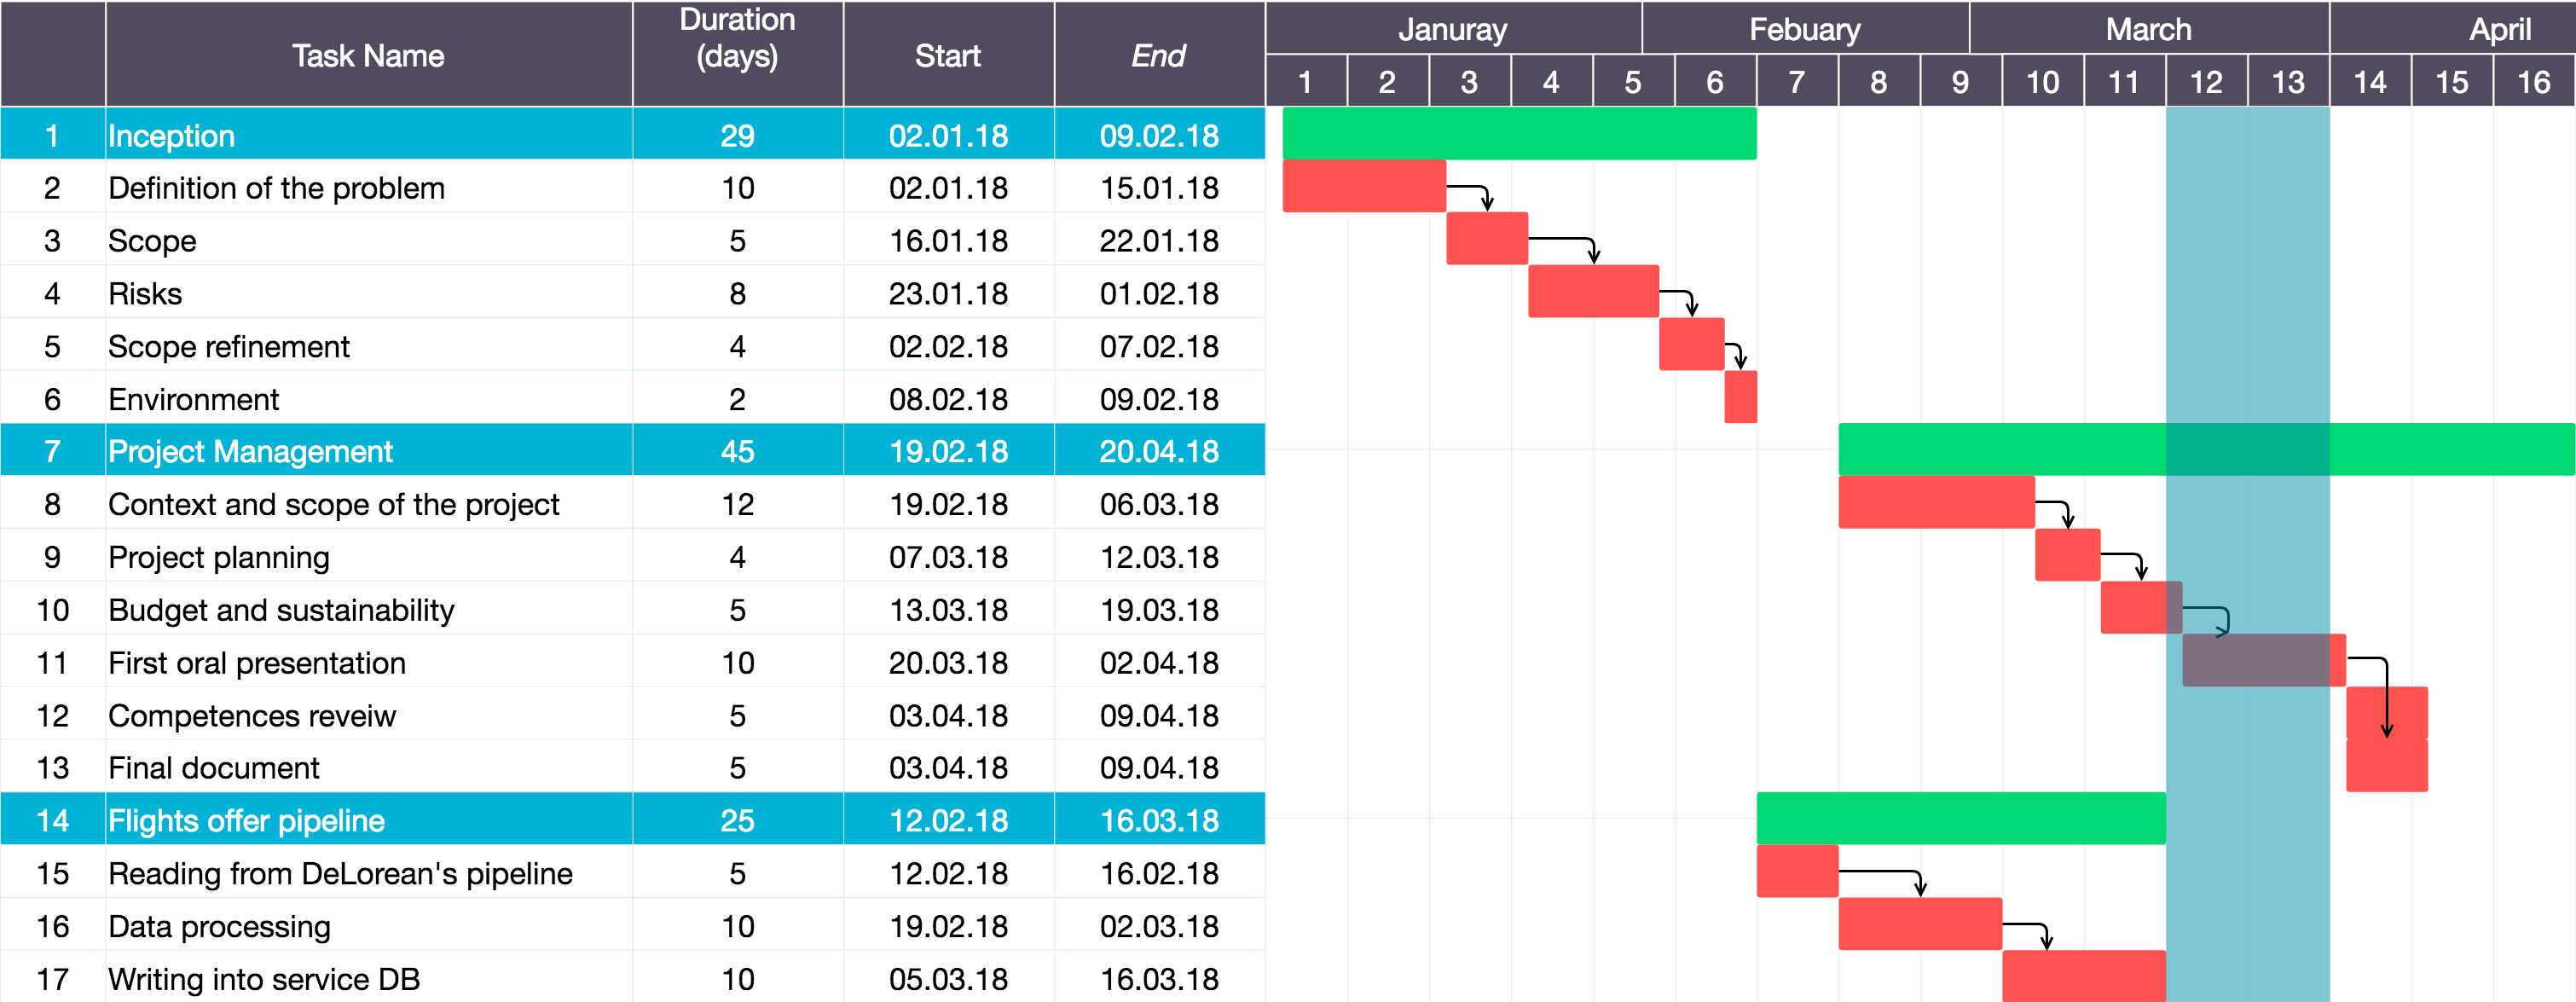
\includegraphics[scale=0.14]{diagrams/gantt01-17.png}
\caption{Gantt diagram from task 1 to 17}
\end{figure}

\begin{figure}[H]
%\centering
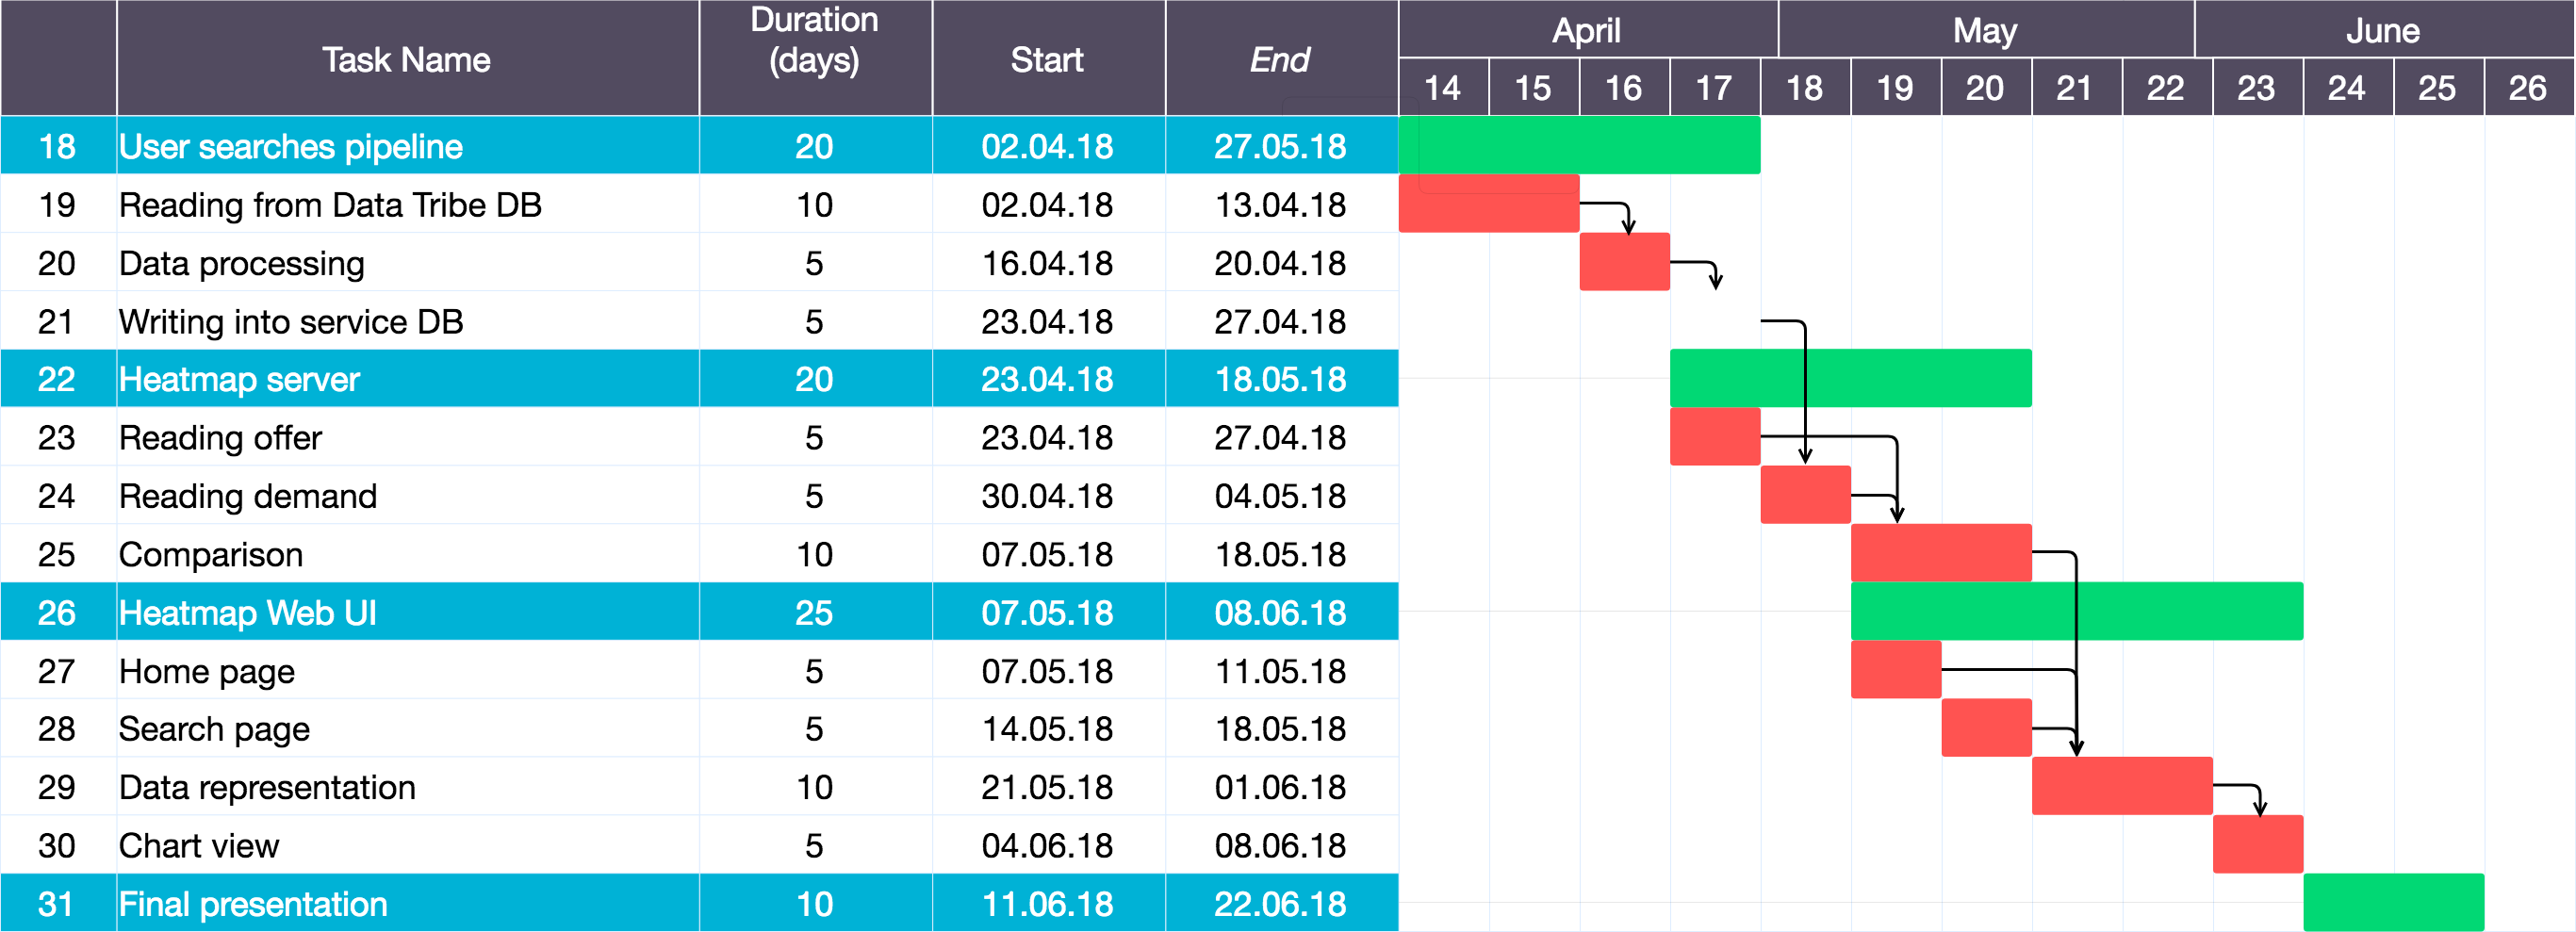
\includegraphics[scale=0.14]{diagrams/gantt18-31.png}
\caption{Gantt diagram from task 18 to 31}
\end{figure}

\begin{figure}[H]
\centering
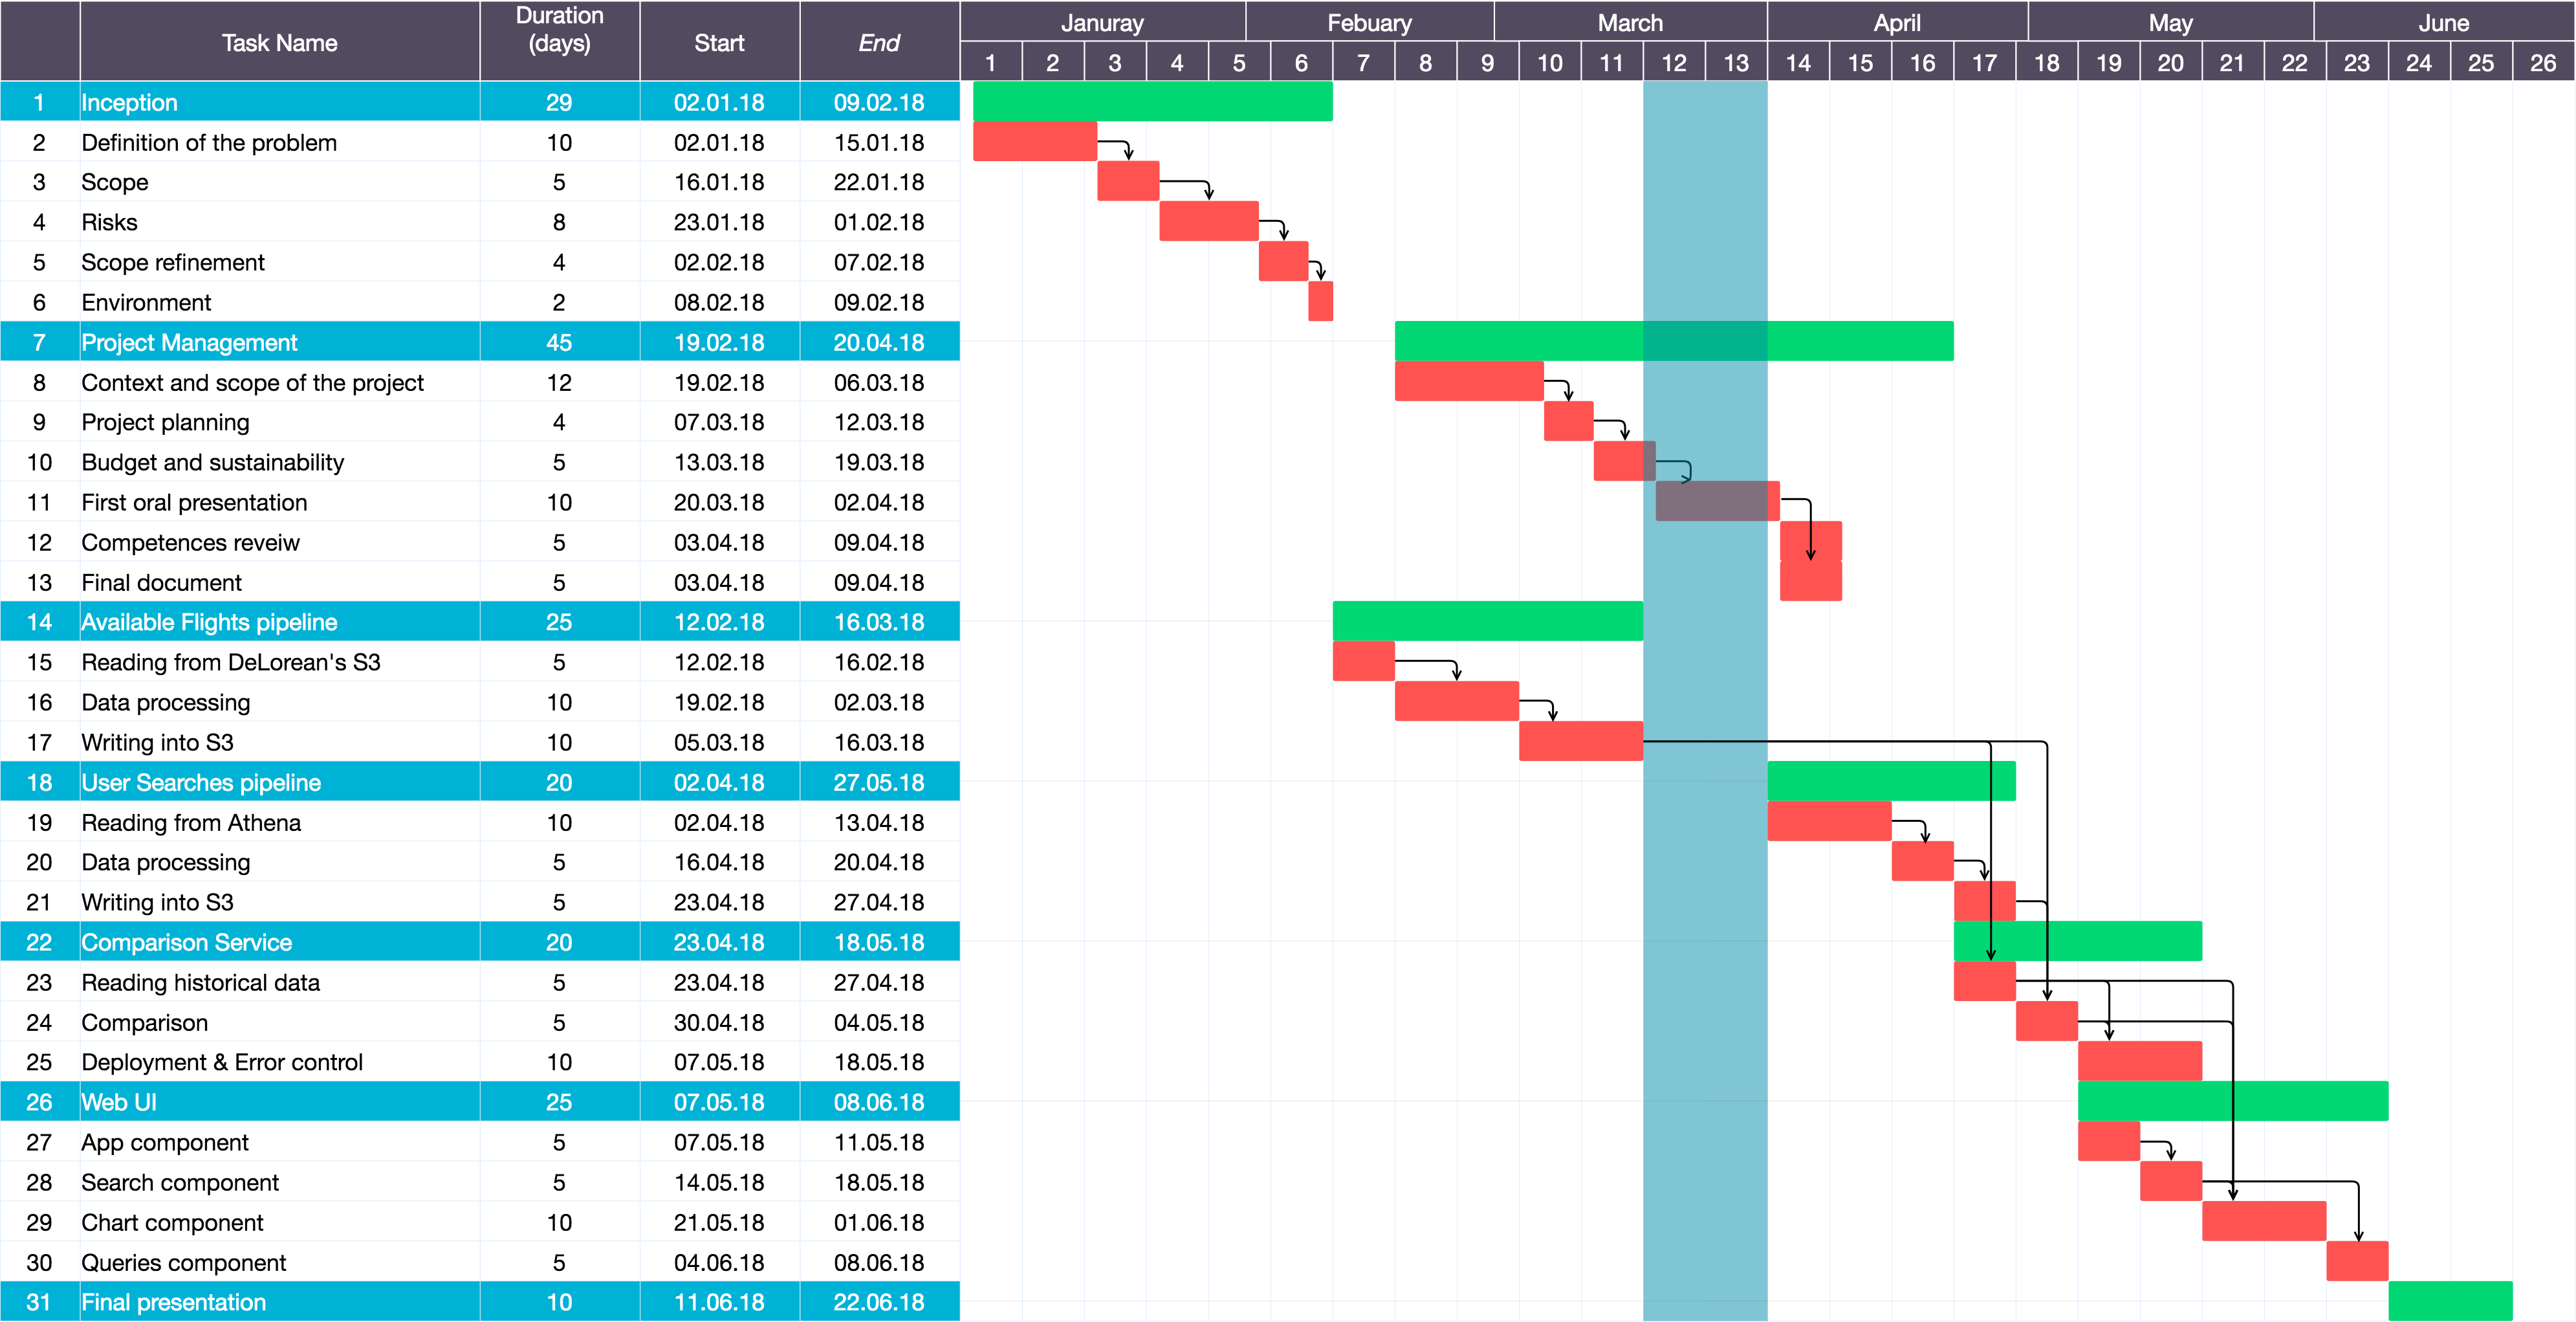
\includegraphics[scale=0.15, angle=270]{diagrams/gantt.png}
\caption{Complete Gantt diagram}
\end{figure}




% Chapter 10: Budget and sustainability

\chapter{Budget and Sustainability}

\label{chapter10}

\section{Budget}

Once the project is planned in time and its technologies are drafted, we can calculate the project’s budget. Skyscanner is not economically transparent, even for the employees. So, this whole calculation will be approximated.
\\\\
First of all, we have to take into account the employees, which is only one and in Intern position, and also count the taxes.
\\\\
Apart from that, all the hardware material and software licenses. AWS costs will continue increasing after the deployment, but since it is going to be used during the development for testing it is counted in the total budget.

\begin{table}[H]
\centering
\begin{tabular}{|l|l|l|l|l|}
\hline
\textbf{Concept}           & \textbf{Price per unit} & \textbf{Units} & \textbf{Amortization} & \textbf{Total £}   \\ \hline
\textbf{Salary}            & 28 (taxes included)     & 575 h          &                       & 16100              \\ \hline
\textbf{MacBook Pro}       & 1700                    & 1              & life cycle 8 years    & 210                \\ \hline
\textbf{JetBrains License} & 230                     & 1              & 1 year per developer  & 115                \\ \hline
\textbf{AWS S3}            & 0.023                   & 50 TB          &                       & 1150               \\ \hline
\textbf{AWS}               & EC2                     & 575 h          &                       & 213.325            \\ \hline
\textbf{Screen}            & 200                     & 2              & life cycle 4 years    & 100                \\ \hline
\textbf{Office}            & Uknown                  & 1              &                       & Uknown             \\ \hline
\textbf{TOTAL}             &                         &                &                       & \textbf{17888.325} \\ \hline
\end{tabular}
\caption{Budget calculation}
\label{budget-calculation}
\end{table}

\section{Sustainability}

\subsection{Economical}

In economic terms, this project is initially unsustainable. It uses resources from Skyscanner for a comparison that might be useful in the future for other projects, improving some services or advertisement.
\\\\
But, if this product is sell to providers, Skyscanner can take a lot of profit from them. It is a very valuable application for providers, since they could compare airlines offer with actual user demand. Letting them improve their flights distribution and make more money.

\subsection{Social}

The \thesis is not directly involving society, but, as explained before, if providers have access to the comparison, flights will improve in terms of traveler experience. Travelers will have accurate routes depending on what they really want.
\\\\
For example, imagine that X carrier have several flights from BCN to ORY, Paris, and a few from BCN to FCO, Rome. The \thesis shows that the demand, compared with the offer is bigger in Rome than in Paris. Then, X airline could schedule more flights to FCO instead of ORY.

\subsection{Environment}

The environmental impact of the \thesis is directly related with the social impact.
\\\\
Right now, some airlines may have half full flights. This means that the airplane is not taking its most advantage of the fuel. It could be carrying more people.
\\\\
If carriers know where flights are really needed those flight will be full of people, which means that the fuel a flight uses is profited at its most.
\\\\
Otherwise, if an offer is under requested, the flight is not giving all the profit it could. In other words, fuel per person will decrease.

\subsection{Sustainability matrix}

In order to understand the general impact of the project, the following general rating and evaluation is provided:
\\\\
The economical impact will be rated in 7/10. It could be a 10/10 it is sell to providers. Air companies could pay a lot of money for the \thesis because of the information it provides.
\\\\
The social impact will get a 4/10. It does nothing good nor bad to the society, only if the application is sell to providers and they use it properly, it could make some good to the people. In the other hand, the software will not be free, it will be property of \company.
\\\\
The environmental impact is a 4/10 as well. The environmental impact could be good if the application is sell to providers and they use it properly, but for now will not be sell to anyone. It gets a 4 because it will be using Amazon Web Service, and those machines are powered mainly by non-renewable energy\cite{click_clean}.
\\\\

\begin{table}[H]
\centering
\begin{tabular}{|l|l|l|}
\hline
Economical & Social & Environmental \\ \hline
7/10       & 4/10   & 4/10          \\ \hline
\multicolumn{3}{|c|}{15/30}         \\ \hline
\end{tabular}
\caption{Sustainability matrix}
\label{sustainability-matrix}
\end{table}


%-------------------------
% CHAPTER 11: Conclusions
%-------------------------

\chapter{Conclusions} \label{chapter11}

After almost six months of the development of a full stack project and after the whole report of the \thesis, there are some conclusions.

\section{Results}

Sadly, results are not the expected, maybe in the beginning the idea was too optimistic thinking that it would be easy to make assumptions when comparing available flights and user searches.
\\\\
From the beginning it was known that one value was for available flights without counting seats of the aircraft or actual \textbf{available seats}, and the other one were searches. Here is an example of why the comparison is not as good as expected:

\begin{figure}[H]
\centering
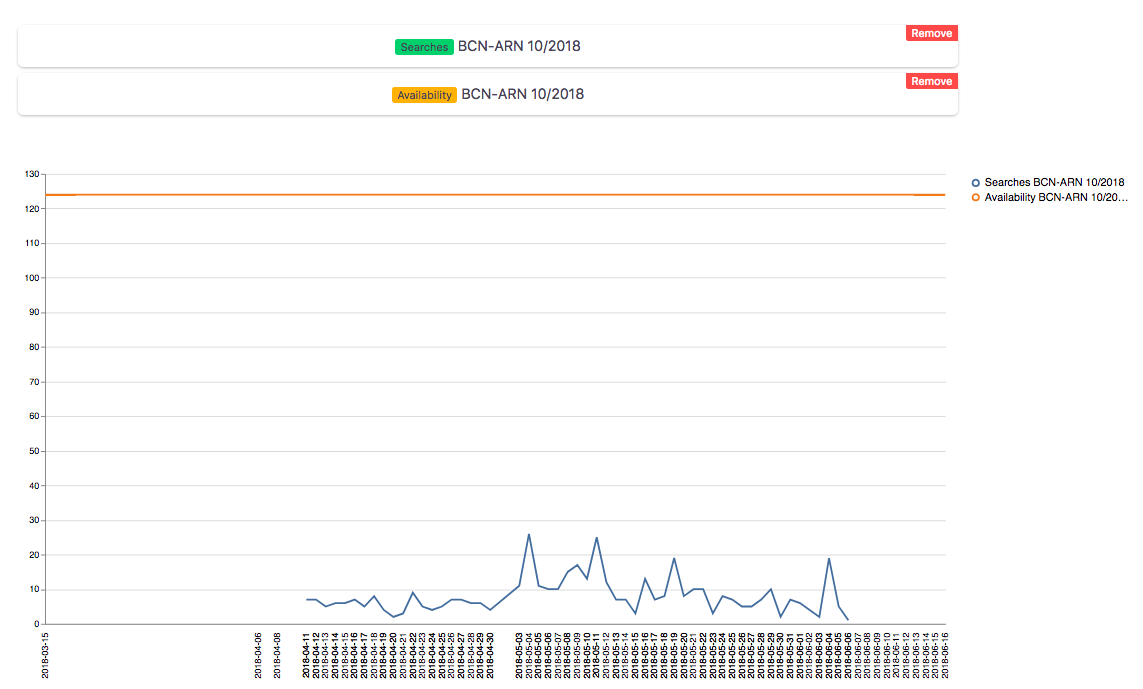
\includegraphics[scale=0.3]{resources/experiment03.png}
\caption{Comparison from Barcelona to Stockholm, October 2018}
\end{figure}

Sometimes, data is not what looks like.
\\\\
Luckily, same source comparisons can give relevant results, see \nameref{exp1} on page \pageref{exp1} and \nameref{exp2} on page \pageref{exp2}.
\\\\
Apart from that issue, all functional and non-functional requirements are fully satisfied. \textbf{The project is completed and works fine}.

\section{Development}

The most valuable thing of this project is the knowledge earned during the making of it. Not only as a programmer, but as a Software Engineer.

\subsubsection*{Inception}

In the beginning looked impossible to find stakeholders and define the project. Being new in the company, was kind of intimidating start talking to product owners. Thanks to my Squad Lead I met them and defined something promising, he set some meetings with product owners he already knew and I end up doing \textbf{elevator pitch}es to them.
\\\\
Now that I am in the end of the project and I know more people and how things work inside of \company, it would be much easier for me to do that process. I would not be afraid of talking to some Product Owners. I can say that \textbf{I learned how to sell a software idea} to anyone, in this case inside the same company.

\subsubsection*{Ping pong}

When specifying and developing the \thesis, if I had some question, I have done \textbf{\textit{ping pong}} between a lot of people. The process is usually the same: You ask something to someone you think they know the answer, but they do not. If you are lucky, they send you to someone that actually knows the answer. But what usually happens next is that they send you to someone they think they know the answer, but they do not neither. The process repeats and repeats until you find the answer.

\subsubsection*{Architecture}

When designing the architecture, I learned a lot. There has been a lot of analysis to different technologies, a lot of alternatives has been studied and discarded, finding a final solution.

\subsubsection*{Methodology}

The agile methodology has been great, but there has been some big blockers that was caused because of the methodology of the company: It took one month to get access to Athena, the ticket I opened to get access to it took a lot of time to be validated and processed.
\\\\
Sometimes it is good to work in a big company because you have a lot of resources that in a start up you cannot get, but for cases like these, you have less \textit{freedom}.

\section{Final conclusion}

It has been great to work in a project of these dimensions. From the beginning until the end.
\\\\
I have learned a lot of great development practices, used different technologies and combined them, I have taken risks always into account and applied different strategies for them and delivered a satisfactory product. I brought something good for Skyscanner.
\\\\
\begin{center}
\textit{The end.}
\end{center}



Special thanks to \textbf{Gary Fernie}, Javier Arias, Francisco Lopez, Esteve Julià, José Durães, Susana Carrera, Jen Agernton

%----------------------------------------------------------------------------------------
\NewPage

% \cleardoublepage
% \phantomsection
\addcontentsline{toc}{chapter}{\listfigurename}
\listoffigures % Prints the list of figures

% \cleardoublepage
% \phantomsection
\addcontentsline{toc}{chapter}{\listtablename}
\listoftables % Prints the list of tables

%----------------------------------------------------------------------------------------
%   BIBLIOGRAPHY
%----------------------------------------------------------------------------------------
\NewPage
\printbibliography[heading=bibintoc]

%----------------------------------------------------------------------------------------
%   THESIS CONTENT - APPENDICES
%----------------------------------------------------------------------------------------
\NewPage
\appendix % Cue to tell LaTeX that the following "chapters" are Appendices

% Include the appendices of the thesis as separate files from the Appendices folder
% Uncomment the lines as you write the Appendices

\chapter{\company\ structure} 

\label{appendix_a}

\company\ has a very horizontal structure, based on Spotify's\cite{culture_of_growth}.
\\\\
In the top of the company hierarchy there is Gareth Williams (CEO and Co-founder). Bellow the rest of CxOs: CCO, CTO, CPO, CFO, CLO and the Senior Executive Assistant. Then vice presidents, senior managers, managers and then developers and interns\cite{crew_chart}.
\\\\
Apart from this hierarchy structure, the whole team, except the CEO, CxOs and the Senior Executive Assistant, is mainly split in \textbf{Squads}, each of those belong to a \textbf{Tribes}. Apart from Squads and Tribes there are also Chapters, Guilds ans XBT'S\cite{how_skyscanner_works}.

\section{Squad}

Are independent teams of no more than 8 people that are focused on delivering a core mission. Each squad has the freedom to act and be accountable to its mission.

\section{Tribe}

Squads belong to a Tribe. The tribe will have an aligning mission linking to each squad's mission and is only achievable depending on the success of each squad. The Tribe lead is responsible for providing the right environment to deliver and providing direction. 

\section{Chapters}

Are people who do similar work. This is a secondary home, and how people are line managed. Chapter leads are responsible for developing people and in tribe practices.

\section{Guilds}

Are communities of interest of people who do not necessarily do similar work. It is people from across the business that want to share knowledge, tools, and word practices. 

\section{XBT'S (cross business teams)}

XBTS' provide a platform to help solve business problems or opportunities with no natural home while giving all employees the ability to make an impact across any area of \company.
\NewPage
\chapter{Design Patterns} 

\label{appendix_b}

Extract from the Design Patterns: Elements of Reusable Object-Oriented Software\cite{design_patterns}.

\section{Singleton}

\subsection*{Intent}

Ensure a class only has one instance, and provide a global point of access to it.

\subsection*{Motivation}

It's important for some classes to have exactly one instance. Although there can be many printers in a system, there should be only one printer spooler. There should be only one file system and one window manager. A digital filter will have one A/D converter. An accounting system will be dedicated to serving one company.
\\\\
How do we ensure that a class has only one instance and that the instance is easily accessible? A global variable makes an object accessible, but it doesn't keep you from instantiating multiple objects.
\\\\
A better solution is to make the class itself responsible for keeping track of its sole instance. The class can ensure that no other instance can be created (by intercepting requests to create new objects), and it can provide a way to access the instance. This is the Singleton pattern.

\subsection*{Applicability}

Use the Singleton pattern when

\begin{itemize}
    \item there must be exactly one instance of a class, and it must be accessible to clients from a well-known access point.
    \item when the sole instance should be extensible by subclassing, and clients should be able to use an extended instance without modifying their code.
\end{itemize}

\subsection*{Structure}

\begin{figure}[H]
\centering
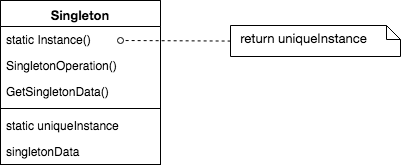
\includegraphics[scale=0.6]{diagrams/singleton.png}
\end{figure}

\subsection*{Participants}

\begin{itemize}
    \item Singleton
    \begin{itemize}
        \item defines an Instance operation that lets clients access its unique instance. Instance is a class operation (that is, a class method in Smalltalk and a static member function in C++).
        \item may be responsible for creating its own unique instance.
    \end{itemize}
\end{itemize}

\subsection*{Collaborations}

\begin{itemize}
    \item Clients access a Singleton instance solely through Singleton's Instance operation.
\end{itemize}

\subsection*{Consequences}

The Singleton pattern has several benefits:

\begin{enumerate}
    \item Controlled access to sole instance. Because the Singleton class encapsulates its sole instance, it can have strict control over how and when clients access it.
    \item Reduced name space. The Singleton pattern is an improvement over global variables. It avoids polluting the name space with global variables that store sole instances.
    \item Permits refinement of operations and representation. The Singleton class may be subclassed, and it's easy to configure an application with an instance of this extended class. You can configure the application with an instance of the class you need at run-time.
    \item Permits a variable number of instances. The pattern makes it easy to change your mind and allow more than one instance of the Singleton class. Moreover, you can use the same approach to control the number of instances that the application uses. Only the operation that grants access to the Singleton instance needs to change.
    \item More flexible than class operations. Another way to package a singleton's functionality is to use class operations (that is, static member functions in C++ or class methods in Smalltalk). But both of these language techniques make it hard to change a design to allow more than one instance of a class. Moreover, static member functions in C++ are never virtual, so subclasses can't override them polymorphically.
\end{enumerate}

\section{Adapter}

Also known as Wrapper.

\subsection*{Intent}

Convert the interface of a class into another interface clients expect. Adapter lets classes work together that couldn't otherwise because of incompatible interfaces.

\subsection*{Motivation}

Sometimes a toolkit class that's designed for reuse isn't reusable only because its interface doesn't match the domain-specific interface an application requires.
\\\\
Consider for example a drawing editor that lets users draw and arrange graphical elements (lines, polygons, text, etc.) into pictures and diagrams. The drawing editor's key abstraction is the graphical object, which has an editable shape and can draw itself. The interface for graphical objects is defined by an abstract class called Shape. The editor defines a subclass of Shape for each kind of graphical object: a LineShape class for lines, a PolygonShape class for polygons, and so forth.
\\\\
Classes for elementary geometric shapes like LineShape and PolygonShape are rather easy to implement, because their drawing and editing capabilities are inherently limited. But a TextShape subclass that can display and edit text is considerably more difficult to implement, since even basic text editing involves complicated screen update and buffer management. Meanwhile, an off-the-shelf user interface toolkit might already provide a sophisticated TextView class for displaying and editing text. Ideally we'd like to reuse TextView to implement TextShape, but the toolkit wasn't designed with Shape classes in mind. So we can't use TextView and Shape objects interchangeably.
\\\\
How can existing and unrelated classes like TextView work in an application that expects classes with a different and incompatible interface? We could change the TextView class so that it conforms to the Shape interface, but that isn't an option unless we have the toolkit's source code. Even if we did, it wouldn't make sense to change TextView; the toolkit shouldn't have to adopt domain-specific interfaces just to make one application work.
\\\\
Instead, we could define TextShape so that it adapts the TextView interface to Shape's. We can do this in one of two ways: (1) by inheriting Shape's interface and TextView's implementation or (2) by composing a TextView instance within a TextShape and implementing TextShape in terms of TextView's interface. These two approaches correspond to the class and object versions of the Adapter pattern. We call TextShape an adapter.

\begin{figure}[H]
\centering
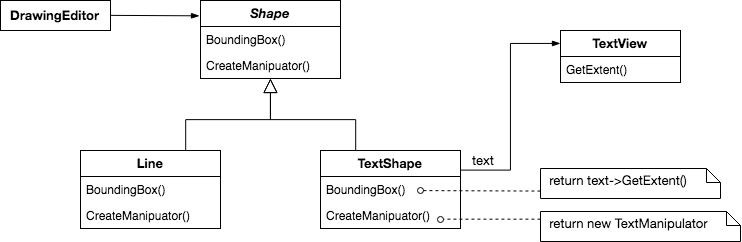
\includegraphics[scale=0.5]{diagrams/adapter_motivation.png}
\end{figure}

This diagram illustrates the object adapter case. It shows how BoundingBox requests, declared in class Shape, are converted to GetExtent requests defined in TextView. Since TextShape adapts TextView to the Shape interface, the drawing editor can reuse the otherwise incompatible TextView class.
\\\\
Often the adapter is responsible for functionality the adapted class doesn't provide. The diagram shows how an adapter can fulfill such responsibilities. The user should be able to "drag" every Shape object to a new location interactively, but TextView isn't designed to do that. TextShape can add this missing functionality by implementing Shape's CreateManipulator operation, which returns an instance of the appropriate Manipulator subclass.
\\\\
Manipulator is an abstract class for objects that know how to animate a Shape in response to user input, like dragging the shape to a new location. There are subclasses of Manipulator for different shapes; TextManipulator, for example, is the corresponding subclass for TextShape. By returning a TextManipulator instance, TextShape adds the functionality that TextView lacks but Shape requires.

\subsection*{Applicability}

Use the Adapter pattern when
\begin{itemize}
    \item you want to use an existing class, and its interface does not match the one you need.
    \item you want to create a reusable class that cooperates with unrelated or unforeseen classes, that is, classes that don't necessarily have compatible interfaces.
    \item (object adapter only) you need to use several existing subclasses, but it's impractical to adapt their interface by subclassing
\end{itemize}

\subsection*{Structure}

A class adapter uses multiple inheritance to adapt one interface to another:

\begin{figure}[H]
\centering
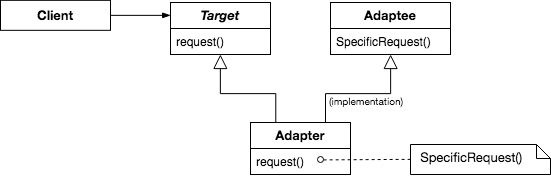
\includegraphics[scale=0.7]{diagrams/adapter_structure_a.png}
\end{figure}

An object adapter relies on object composition:

\begin{figure}[H]
\centering
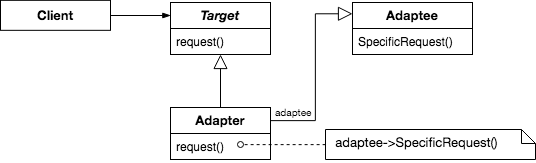
\includegraphics[scale=0.7]{diagrams/adapter_structure_b.png}
\end{figure}

\subsection*{Participants}

\begin{itemize}
    \item Target (Shape)
    \begin{itemize}
        \item defines the domain-specific interface that Client uses.
    \end{itemize}
    \item Client (DrawingEditor)
    \begin{itemize}
        \item collaborates with objects conforming to the Target interface.
    \end{itemize}
    \item Adaptee (TextView)
    \begin{itemize}
        \item defines an existing interface that needs adapting.
    \end{itemize}
    \item Adapter (TextShape)
    \begin{itemize}
        \item adapts the interface of Adaptee to the Target interface.
    \end{itemize}
\end{itemize}

\subsection*{Collaborations}

\begin{itemize}
    \item Clients call operations on an Adapter instance. In turn, the adapter calls Adaptee operations that carry out the request.
\end{itemize}

\subsection*{Consequences}

Class and object adapters have different trade-offs. A class adapter
\begin{itemize}
    \item adapts Adaptee to Target by committing to a concrete Adapter class. As a consequence, a class adapter won't work when we want to adapt a class and all its subclasses.
    \item lets Adapter override some of Adaptee's behavior, since Adapter is a subclass of Adaptee.
    \item introduces only one object, and no additional pointer indirection is needed to get to the adaptee.
\end{itemize}

An object adapter
\begin{itemize}
    \item lets a single Adapter work with many Adaptees—that is, the Adaptee itself and all of its subclasses (if any). The Adapter can also add functionality to all Adaptees at once.
    \item makes it harder to override Adaptee behavior. It will require subclassing Adaptee and making Adapter refer to the subclass rather than the Adaptee itself.
\end{itemize}

Here are other issues to consider when using the Adapter pattern:
\begin{enumerate}

    \item How much adapting does Adapter do? Adapters vary in the amount of work they do to adapt Adaptee to the Target interface. There is a spectrum of possible work, from simple interface conversion—for example, changing the names of operations—to supporting an entirely different set of operations. The amount of work Adapter does depends on how similar the Target interface is to Adaptee's.

    \item Pluggable adapters. A class is more reusable when you minimize the assumptions other classes must make to use it. By building interface adaptation into a class, you eliminate the assumption that other classes see the same interface. Put another way, interface adaptation lets us incorporate our class into existing systems that might expect different interfaces to the class. ObjectWorks/Smalltalk [Par90] uses the term pluggable adapter to describe classes with built-in interface adaptation.
    \\\\
    Consider a TreeDisplay widget that can display tree structures graphically. If this were a special-purpose widget for use in just one application, then we might require the objects that it displays to have a specific interface; that is, all must descend from a Tree abstract class. But if we wanted to make TreeDisplay more reusable (say we wanted to make it part of a toolkit of useful widgets), then that requirement would be unreasonable. Applications will define their own classes for tree structures. They shouldn't be forced to use our Tree abstract class. Different tree structures will have different interfaces.
    \\\\
    In a directory hierarchy, for example, children might be accessed with a GetSubdirectories operation, whereas in an inheritance hierarchy, the corresponding operation might be called GetSubclasses. A reusable TreeDisplay widget must be able to display both kinds of hierarchies even if they use different interfaces. In other words, the TreeDisplay should have interface adaptation built into it.
    \\\\
    We'll look at different ways to build interface adaptation into classes in the Implementation section.

    \item Using two-way adapters to provide transparency. A potential problem with adapters is that they aren't transparent to all clients. An adapted object no longer conforms to the Adaptee interface, so it can't be used as is wherever an Adaptee object can. Two-way adapters can provide such transparency. Specifically, they're useful when two different clients need to view an object differently.
    \\\
    Consider the two-way adapter that integrates Unidraw, a graphical editor framework [VL90], and QOCA, a constraint-solving toolkit [HHMV92]. Both systems have classes that represent variables explicitly: Unidraw has StateVariable, and QOCA has ConstraintVariable. To make Unidraw work with QOCA, ConstraintVariable must be adapted to StateVariable; to let QOCA propagate solutions to Unidraw, StateVariable must be adapted to ConstraintVariable.
    \begin{figure}[H]
    \centering
    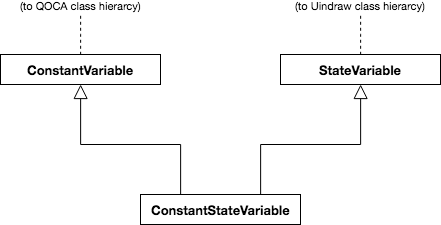
\includegraphics[scale=0.6]{diagrams/adapter_consequence.png}
    \end{figure}
    The solution involves a two-way class adapter ConstraintStateVariable, a subclass of both StateVariable and ConstraintVariable, that adapts the two interfaces to each other. Multiple inheritance is a viable solution in this case because the interfaces of the adapted classes are substantially different. The two-way class adapter conforms to both of the adapted classes and can work in either system.
\end{enumerate}

\section{Composite}

\subsection*{Intent}

Compose objects into tree structures to represent part-whole hierarchies. Composite lets clients treat individual objects and compositions of objects uniformly.

\subsection*{Motivation}

Graphics applications like drawing editors and schematic capture systems let users build complex diagrams out of simple components. The user can group components to form larger components, which in turn can be grouped to form still larger components. A simple implementation could define classes for graphical primitives such as Text and Lines plus other classes that act as containers for these primitives.
\\\\
But there's a problem with this approach: Code that uses these classes must treat primitive and container objects differently, even if most of the time the user treats them identically. Having to distinguish these objects makes the application more complex. The Composite pattern describes how to use recursive composition so that clients don't have to make this distinction.

\begin{figure}[H]
\centering
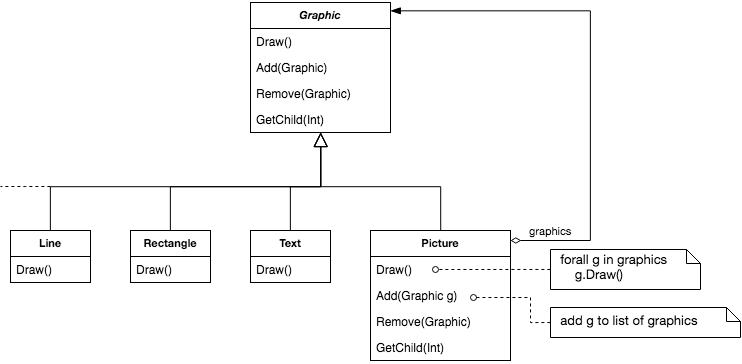
\includegraphics[scale=0.5]{diagrams/composite_motivation.png}
\end{figure}

The key to the Composite pattern is an abstract class that represents both primitives and their containers. For the graphics system, this class is Graphic. Graphic declares operations like Draw that are specific to graphical objects. It also declares operations that all composite objects share, such as operations for accessing and managing its children.
\\\\
The subclasses Line, Rectangle, and Text (see preceding class diagram) define primitive graphical objects. These classes implement Draw to draw lines, rectangles, and text, respectively. Since primitive graphics have no child graphics, none of these subclasses implements child-related operations.
\\\\
The Picture class defines an aggregate of Graphic objects. Picture implements Draw to call Draw on its children, and it implements child-related operations accordingly.
\\\\
Because the Picture interface conforms to the Graphic interface, Picture objects can compose other Pictures recursively.
\\\\
The following diagram shows a typical composite object structure of recursively composed Graphic objects:

\begin{figure}[H]
\centering
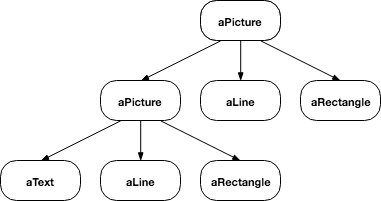
\includegraphics[scale=0.7]{diagrams/composite_motivation_s.png}
\end{figure}

\subsection*{Applicability}

Use the Composite pattern when
\begin{itemize}
    \item you want to represent part-whole hierarchies of objects.
    \item you want clients to be able to ignore the difference between compositions of objects and individual objects. Clients will treat all objects in the composite structure uniformly.
\end{itemize}

\subsection*{Structure}

\begin{figure}[H]
\centering
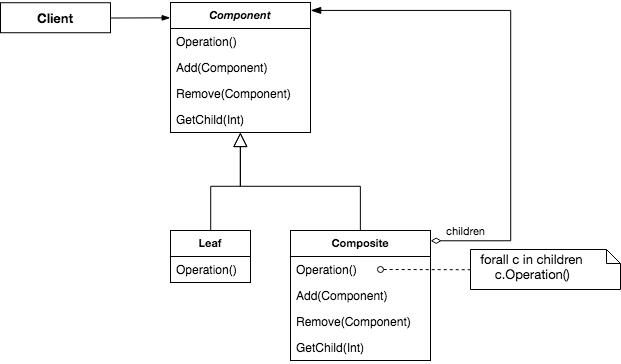
\includegraphics[scale=0.6]{diagrams/composite_structure.png}
\end{figure}

A typical Composite object structure might look like this:

\begin{figure}[H]
\centering
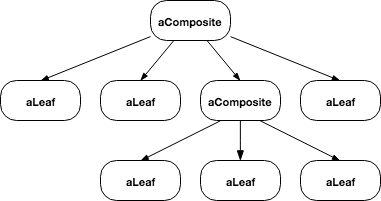
\includegraphics[scale=0.7]{diagrams/composite_structure_s.png}
\end{figure}

\subsection*{Participants}

\begin{itemize}
    \item Component (Graphic)
    \begin{itemize}
        \item declares the interface for objects in the composition.
        \item implements default behavior for the interface common to all classes, as appropriate.
        \item declares an interface for accessing and managing its child components.
        \item (optional) defines an interface for accessing a component's parent in the recursive structure, and implements it if that's appropriate.
    \end{itemize}
    \item Leaf (Rectangle, Line, Text, etc.)
    \begin{itemize}
        \item represents leaf objects in the composition. A leaf has no children.
        \item defines behavior for primitive objects in the composition.
    \end{itemize}
    \item Composite (Picture)
    \begin{itemize}
        \item defines behavior for components having children.
        \item stores child components.
        \item implements child-related operations in the Component interface.
    \end{itemize}
    \item Client
    \begin{itemize}
        \item manipulates objects in the composition through the Component interface.
    \end{itemize}
\end{itemize}

\subsection*{Collaborations}

\begin{itemize}
    \item Clients use the Component class interface to interact with objects in the composite structure. If the recipient is a Leaf, then the request is handled directly. If the recipient is a Composite, then it usually forwards requests to its child components, possibly performing additional operations before and/or after forwarding.
\end{itemize}

\subsection*{Consequences}

The Composite pattern
\begin{itemize}
    \item defines class hierarchies consisting of primitive objects and composite objects. Primitive objects can be composed into more complex objects, which in turn can be composed, and so on recursively. Wherever client code expects a primitive object, it can also take a composite object.
    \item makes the client simple. Clients can treat composite structures and individual objects uniformly. Clients normally don't know (and shouldn't care) whether they're dealing with a leaf or a composite component. This simplifies client code, because it avoids having to write tag-and-case-statement-style functions over the classes that define the composition.
    \item makes it easier to add new kinds of components. Newly defined Composite or Leaf subclasses work automatically with existing structures and client code. Clients don't have to be changed for new Component classes.
    \item can make your design overly general. The disadvantage of making it easy to add new components is that it makes it harder to restrict the components of a composite. Sometimes you want a composite to have only certain components. With Composite, you can't rely on the type system to enforce those constraints for you. You'll have to use run-time checks instead.
\end{itemize}



\end{document} 